\documentclass{scrartcl}

% input encoding
\usepackage[utf8]{inputenc}

% new german spelling
\usepackage[ngerman]{babel}

% choose font
\usepackage[T1]{fontenc}
\usepackage{lmodern}

% KOMA-Script options
\KOMAoptions{%
  parskip=full,%
  fontsize=12pt,
  DIV=calc}

% color and images
\usepackage{xcolor}
\usepackage{graphicx}
\graphicspath{{/Users/Sheraz/Documents/Latex/RechnernetzeDokumentation/Gesamtdoku/Bilder/}}

% quotes
\usepackage[german=guillemets]{csquotes}

% math
\usepackage{amsmath}
\usepackage{ulem}

% set special behaviour for hyperlinks in pdfs
\usepackage[breaklinks=true]{hyperref}


\begin{document}
  \title{Rechnernetze Dokumentation}
  \author{Sheraz Azad und Sven Marquardt}
  \date{Wintersemester 2015/16}
  \maketitle
  
  \tableofcontents
  \textbf{ALLE BILDER UND TABELLEN MÜSSEN IN DEN TEXTFLUSS EINGEBUNDEN WERDEN}
  
%---------------------------------------------------------------------------------------------------------------------------- 
  \newpage
\section[Versuch 1 Schichtenmodell]{Schichtenmodell}  
  \subsection[Aufgabe 2 Überlegungen für das Spiel Vier gewinnt]{Überlegungen für das Spiel ''Vier gewinnt''}
  
  Die Kommunikation untereinander findet mittels einer Münze statt, welche hochgehalten wird, wobei wir den Binärcode verwenden. Zeigt die Münze Kopf stellt diese die 0 dar und zeigt die Münze Zahl stellt sie die 1 dar. Damit die beiden Positionen unterscheidbar sind, wird die Münze pro Position, also entweder Kopf (0) oder Zahl (1), jeweils für 2 Sekunden hochgehalten erst danach findet ein Positionswechsel statt.
    
  Damit eine geregelte und sinnvolle Kommunikation zwischen den Kommunikationspartnern stattfinden kann, wurden Kommunikationsregeln festgelegt. Das Spiel ''Vier gewinnt'' hat 7 Reihen mit jeweils 6 Feldern, da wir bei diesem Spiel nur die Spaltenangabe brauchen um unseren Spielzug zu machen, wurden 3 Bits verwendet von 001 (1) bis 111 (7) welche die einzelnen Spalten darstellen.
  
  \textbf{HIER EIN BILD VON EINEM VIER GEWINNT SPIELFELD}\\
  \textbf{HIER FEHLT NOCH WIE MAN ENTSCHEIDET WER ALS ERSTES DRAN IST}
  
  Weitere Bitcodierungen für die Kommunikation sind:
 %TABELLE SOLL NOCH IM TEXTFLUSS UNTEN SEIN  

    \begin{tabular}{|c|l}
      \textbf{Bitfolge} & \textbf{Bedeutung} \\ \hline
        001 & Reihe voll \\
      110 & Gewonnen \\
      101 & Unentschieden \\
      011 & Weiter \\
      100 & Fertig \\
      111 & Nochmal bei Fehlübertragung 
    \end{tabular}
    
  \textbf{HIER EIN BEISPIEL FÜR DEN SPIELFLUSS DEN ENTWEDER ICH IN LÜBECK HABE}
  
 \begin{table}
    \centering
    \caption{Hybrides Modell}
    \begin{tabular}{l|ll}
      5. Anwendungschicht & Das Spiel ''Vier gewinnt'' \\ \hline
      4. Transportschicht & Wird nicht verwendet \\ \hline
      3. Vermittlungsschicht & Wird nicht verwendet \\ \hline
      2. Sicherungsschicht & Übersetzen der Kommunikation in Bits und Fehlererkennung \\ \hline
      1. Bitübertragungsschicht & Übertragung von 0 und 1 durch Medium Münze\\ 
     \end{tabular}
\end{table}

 \subsection[Aufgabe 4 Vor- und Nachteile der Realisierung]{Vor- und Nachteile der Realisierung}

Zweierteam mit dem die Analyse der Spielrealisierung gemacht wurde bestand aus Malte Grebe und Niklas Klatt. 
 
 \textbf{Vorteile:}\\
 Aufgrund der Kommunikationsregeln ist das Spiel leicht zu verstehen und zu bedienen. Durch die ständige Überprüfung wird dafür gesorgt, das keine Fehler bei der Übertragung auftreten. Dadurch das ein Weiter (011) erwartet wird, gibt es Spielpausen und man kann in Ruhe sein Spielfeld aktualisieren. 
 
 \textbf{Nachteile:}\\
  Ein Zug dauert ca. eine Minute, da jede Position zwei Sekunden gehalten wird. Spieler 1 oder 2 fängt zu früh mit der Übertragung vom nächsten Spielzug an, dadurch gibt es eine Fehlerübertragung die wiederholt werden muss.
  
  \textbf{Verbesserte Spielrealisierung:}\\
  Einführung einer Spielfeldsynchronisierung um sicherzustellen, das keine Fehler beim Eintragen der Positionen eingetreten sind. 
  
  \subsection[Aufgabe 5 Verbesserte Kommunikation durch Stifte]{Verbesserte Kommunikation durch Stifte}
  
  Es gibt zwei Varianten die Kommunikation druch Stifte zu verbessern.
  
  Die \textbf{erste Variante} ist, das man einen waagerechten Sitft als 0 und einen senkrechten Stift als 1 interpretiert. Dadurch lassen sich die drei Kommunikationsbit leicht, schnell und eindeutig darstellen.
  
  \textbf{HIER EINE ZEICHNUNG MIT HALBWINKEL UND DIE BITS ZU DEN WINKELN}
  
  Die \textbf{zweite Variante} ist, dass man die Stifte in bestimmten Winkel hinlegt. Hier können wir zum Beispiel sagen das wenn der Stift in einem 90 Grad Winkel liegt, dieser die Bitfolge 001 für Reihe voll darstellt. So können wir die verschiedenen Bitfolgen angeben und bräuchten mit dieser Variante sogar nur einen Stift statt drei.
  
  Diese Fragestellung bezieht sich auf die Bitübertragungsschicht, da sie für die Übertragung von Informationen (Bits 0 und 1) zuständig ist.
  
   \subsection[Aufgabe 6 Kommunikation durch Klatschen]{Kommunikation durch Klatschen}
   
   \textbf{Problem}\\
   Dadurch das alle Teams zeitgleich angefangen haben zu klatschen, konnte man nicht unterscheiden ob das Klatschgeräusch vom gegenüber sitzenden Kommunikationspartner kam, oder von einem Kommilitonen aus einer anderen Gruppe. Aufgrund dieser Tatsache sind bei allen Teams Fehler bei der Kommunikation entstanden.
   
   \textbf{Lösung}\\
   Auch hier gibt es zwei Lösungsansätze, die sich auf die Medienzugriffskontrollte aufbauen, in der dann nur eine Gruppe zur Zeit kommunizieren darf. Diese Möglichkeiten sind.
   
   \textbf{1. Ohne Koordinator:} Jeder Gruppe im Raum wird eine zufällige Wartezeit in Sekunden zugeteilt, die sie abwarten müssen um kommunizieren zu können. Tritt der Fall auf das zwei oder mehrere Gruppen zur selben Zeit kommunizieren wollen, wird eine Wartezeit aus einem größeren Zeitintervall genommen um diesen Fall zu umgehen. Je nach Wichtigkeit könnte man hier den jeweiligen Gruppen eine Wartezeit aus einem kleinen Zeitintervall zu weisen, als dem Rest der Gruppen.
   
   \textbf{2. Mit Koordinator:} Bei diesem Lösungansatz gibt es einen Koordinator im Raum, der die Anfragen der Gruppen, die kommunizieren wollen, an sich nimmt und stellt dann eine nach seinen Kriterien faire Reihenfolge fest, in der die Gruppen dann untereinander kommunizieren dürfen. Die Reihenfolge hängt natürlich je nach Wichtigkeit der Gruppen ab und wird vom Koordinator behandelt.
   
   Diese Fragestellung bezieht sich auf die Sicherungsschicht, da sie für die zuverlässige Übertragung von Informationen von einem Teilnehmer zum anderen Teilnehmer zuständig ist.
   
    \subsection[Aufgabe 7 Kommunikation mit beliebigen Teilnnehmern]{Kommunikation mit beliebigen Teilnnehmern}
    
    Wenn man davon ausgeht das jeder Teilnehmer dieselben Kommunikationsregeln hat, vergibt man jedem Teilnehmer eine eindeutige Adresse. Möchte man nun einen anderen Teilnehmer kontaktieren, muss man die zu übermittelende Nachricht adressieren. Die beinhaltenden Informationen der Nachricht bestehen aus Sender, Empfänger und Nachricht. Hierbei muss beachtet werden, das bevor man den Kontakt zu einem Teilnehmer aufnehmen möchte, vor Beginn des Spiels eine Kontaktaufnahme erfolgen muss die vom Empfänger bestätigt wird und erst dann kann das Spiel beginnen.
    
    Diese Fragestellung bezieht sich ebenfalls auf die Sicherungsschicht, da sie für die zuverlässige Übertragung von Informationen von einem Teilnehmer zum anderen Teilnehmer zuständig ist.
    
    \subsection[Aufgabe 8 Kommunikation mit bestimmten Teilnehmern]{Kommunikation mit bestimmten Teilnehmern}
    
    Auch hier bekommt jeder Teilnehmer eine \textbf{eindeutige} Adresse, wobei diese jedoch noch die Informationen Gebäude-, Raum-, Reihen- und Sitznummer beinhalten. Die Nachricht wird somit anhand dieser ausführlichen Informationen an den jeweiligen Teilnehmer gesendet.
    
    Diese Fragestellung bezieht sich auf die Vermittlungsschicht, da jeder Teilnehmer aufgrund der eindeutigen Adresse mit jedem anderenen (bestimmten) Teilnehmer kommunizieren kann.
    
     \subsection[Aufgabe 9 Datenfluss Problem]{Datenfluss Problem}
     
     \textbf{Problem}\\
     Bei einem worst-case-scenario erhält ein spezieller Teilnehmer soviele Informationen von anderen Teilnehmern, das er keinen Platz bzw keine Zeit mehr hat sich die Informationen zu notieren. Folglich gehen dadurch Informationen verloren und diese werden ein weiteres mal an denselben Teilnehmer gesendet, welches das Problem in die Länge zieht.
     
     \textbf{Lösung}\\
     Um den Informationsfluss zu stoppen oder zu kontrollieren schickt der spezielle Teilnehmer bei Bedarf eine Nachricht an die Teilnehmer das diese entweder langsamer senden sollen oder nur eine bestimmte Anzahl an Informationen senden dürfen. Bleibt das Problem weiterhin bestehen, schickt der spezielle diese Nachricht solange bis der Informationsfluss für ihn verarbeitbar ist.
     Außerdem können weitere spezielle Teilnehmer eingeteilt werden um den Informationsfluss an mehrere spezielle Teilnehmer zu verteilen und dadurch den Arbeitsaufwand eines speziellen Teilnehmers zu senken.
     
     Diese Fragestellung bezieht sich auf die Transportsschicht, da es sich hierbei um eine Staukontrolle handelt, damit ein Teilnehmer seine Informationsrate zu schicken mindert, wenn das Netz überlastet ist.

%----------------------------------------------------------------------------------------------------------------------------
  \newpage
\section[Versuch 2 Zuverlässige Datenübertragung]{Zuverlässige Datenübertragung}
  \subsection[Aufgabe 2 Messung der Häufigkeit von Rahmenverlusten]{Messung der Häufigkeit von Rahmenverlusten}
  
  Jedes mal wenn der Client einen Rahmen sendet erhöht der Server einen Counter für einen empfangenen Rahmen um eins. Nachdem die Übertragung statt gefunden hat, kann der Server nun überprüfen ob es einen Rahmenverlust gab, indem er die Datei aufruft und die Differenz zwischen der Länge der Datei und dem Counter berechnet. \\
Rahmen insgesamt - Empfangene  Rahmen = Verlorene Rahmen.\\
Wenn die Differenz null beträgt, dann ist kein Rahmenverlust aufgetreten.

  \subsection[Aufgabe 3 Messung der Bitfehlerrate]{Messung der Bitfehlerrate}
 
  \subsection[Aufgabe 4 Vorüberlegungen zum sicheren Protokoll]{Vorüberlegungen zum sicheren Protokoll}
  
  Um Rahmenverluse und Bitfehler zu kompensieren, gibt es viele Möglichkeiten, wobei folgende Maßnahmen in der zu diesem Pariktum zugehörigen Vorlesung und in anderen Vorlesungen wie Verteile Systeme vorgestellt wurden.
  
    \begin{enumerate}
    \item Die einfachste Möglichkeit ist einen \textbf{Timer} bei senden von Daten zu starten, welcher auf der Serverseite implementiert wird. Wenn nach einer bestimmten keine Rückmeldung vom Client empfangen wird, dann schickt der Server dieses Datenpaket noch einmal. Die Rückmeldung ist das Prinzip der Quittungen (Acknowledgements), welche entweder postiv (Datenpaket angekommen) oder negativ (Datenpaket nicht angekommen) sein können.
    \item Passend zu dem Prinzip der oben genannten Quittungen, könnte man auch das dazu passende \textbf{Stop-and-Wait Protokoll} implementieren. Hierbei darf der Sender nur dann ein Datenpaket senden, wenn er von dem zuvor gesendeten Datenpaket eine Quittung vom Empfänger erhält. Falls die Quittung negativ ist wird das Datenpaket erneut gesendet, ansonsten das nächste Datenpaket welches an der Reihe ist, wie oben schon erwähnt wurde.
    \item Um Duplikate zu verhindern kann man \textbf{Sequenznummern} verwenden. Wenn z.B. die Quittung vom Empfänger an den Sender verloren geht und dieser nach dem Tiemout das Datenpaket erneut sendet, hat der Empfänger redundante Datenpakete. Dieser kann dann anhand der Sequenznummern das er dieses Datenpaket schon empfangen hat, verwirft das zweite redundante Datenpaket und verschickt erneut eine positive Quittung an den Sender. 
    \item Eine weitere Methode ist es ein \textbf{Paritätsbit} (Parity byte) zu verwenden. Dieses Paritätsbit wird an die Bits des Datenpakets angehängt und berechnet sich aus der Summe aller Bits. Wenn die Summer der Bits gerade ist, ist das Paritätsbit ''0'', ist die Summe jedoch ungerade, ist das Paritätsbit ''1''. Das Problem mit dem Paritätsbit jedoch ist das Fehler eventuell nicht entdeckt werden. Haben wir zum Beispiel Bytefolge ''01000001'' ergibt sich das Paritätsbit ''0'' dafür. Entstehen hier jedoch zum Beispiel zwei Bitfehler wird aus der Bytfolge ''10000010'', die Bytefolge ''10101010'' aus dem sich ebenfalls das Paritätsbit ''0'' berechnen lässt. Allgemein bedeutet das, dass sich eine gerade Anzahl von Fehlern aufhebt und nur eine ungerade Anzahl von Fehlern das Paritätsbit ändert. 
  \end{enumerate}
  
  \subsection[Aufgabe 6 Verhinderung von Rahmenverlusten]{Verhinderung von Rahmenverlusten}

%----------------------------------------------------------------------------------------------------------------------------  
  \newpage
\section[Versuch 3 Anwendungsschicht und Tools]{Anwendungsschicht und Tools}

  \subsection[Aufgabe 4 nslookup tool]{nslookup tool}
  
  (Verwendet wurde das Terminal von einem MacBook Pro mid 2014 mit dem OS El Captian)
 
  \begin{figure}
  \centering
    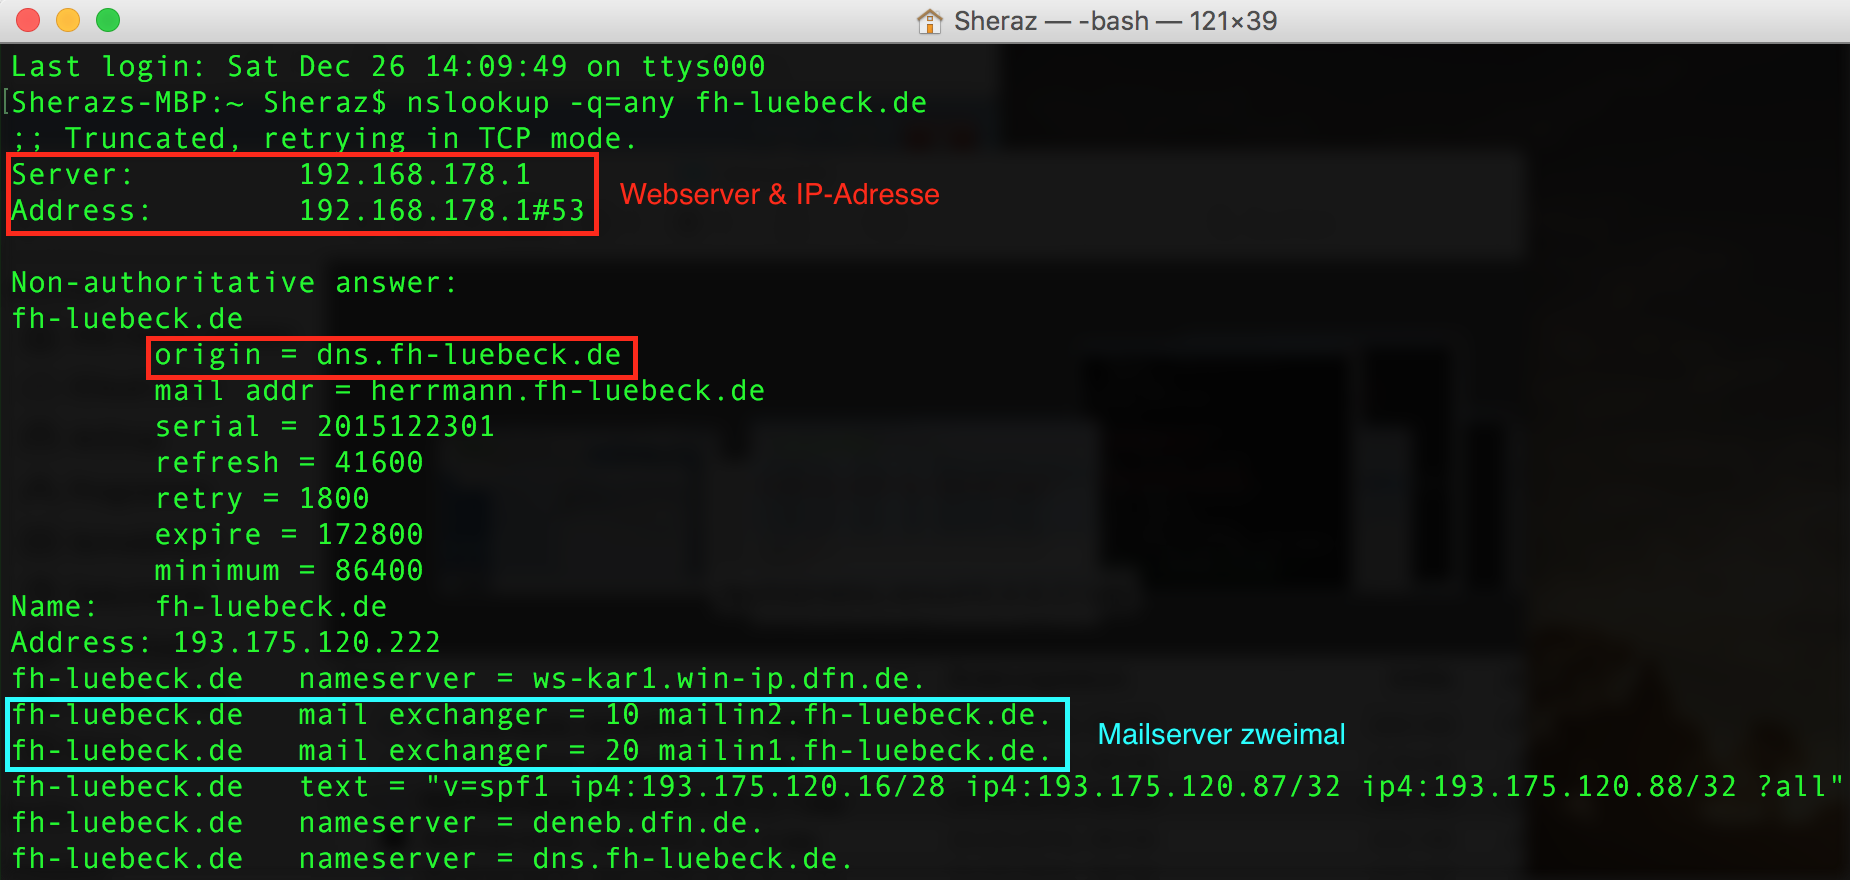
\includegraphics[width=15cm]{nslookup}
    \label{fig:nslookup}
  \end{figure}

  \begin{figure}
  \centering
    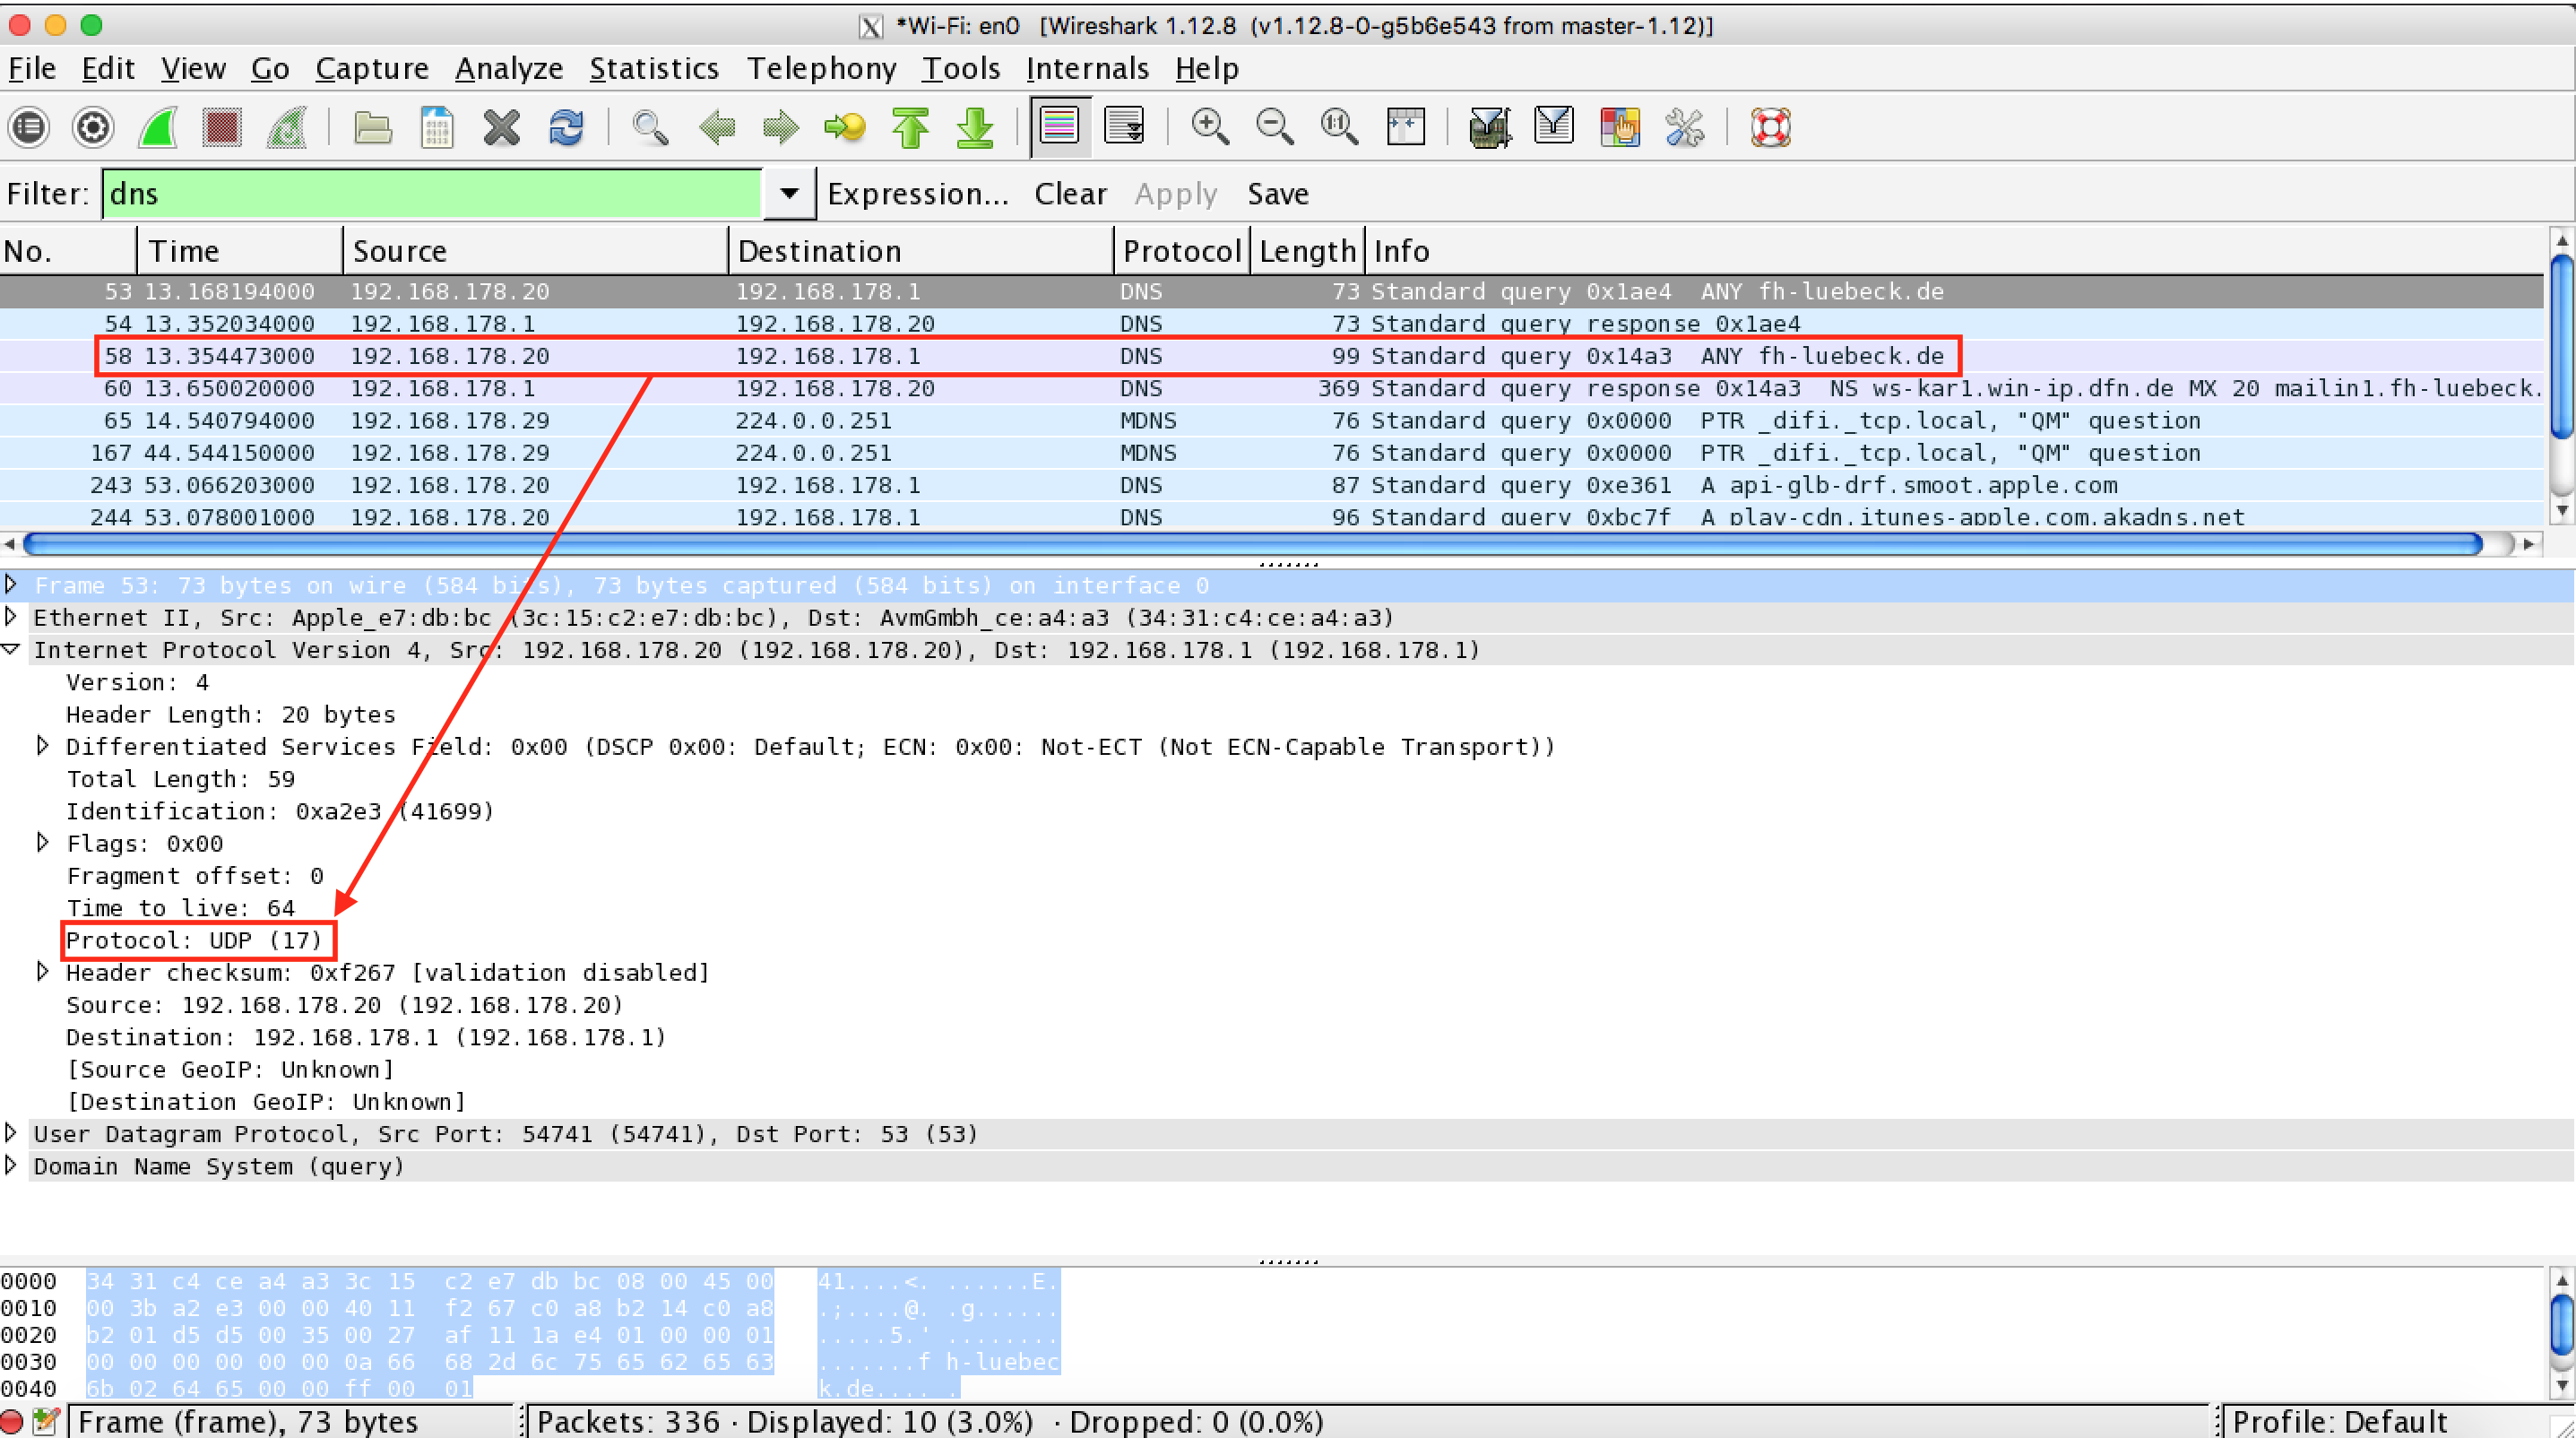
\includegraphics[width=15cm]{wirensany}
    \label{fig:wirensany}
  \end{figure}  
  

  Bei dem Befehl \textbf{nslookup -q = any fh-luebeck.de} erhält man die IP-Adresse \textit{192.168.178.1} für den Server und \textit{fh-luebeck.de mail exchanger = 20 mailin1.fh-luebeck.de. und fh-luebeck.de mail exchanger = 10 mailin2.fh-luebeck.de.} für die Mail Server. 
  
  Aufgrund einer Aktualisierung konnte mit dem Befehl \textbf{nslookup -q = any fh-luebeck.de 8.8.8.8 / 8.8.4.4} konnte keine Unterschied weder am Macbook noch an den Laborrechnern festgestellt werden. Aus Neugier wurden Informationen bezüglich des Unterschiedes der beiden Anfragen, von Kommilitonen aus dem höheren Semester nachgefragt. Der offensichtliche Unterschied der beiden Anfragen ist, dass beim zweiten Befehl nicht nur der Hostname-Parameter sondern auch der Server-Parameter eingegeben wurde. 8.8.8.8/8.8.4.4 ist ein öffentlich zugänglicher DNS Server von Google, der auch Informationen über die FH-Lübeck gespeichert hat, welche wir dann über diesen öffentlichen DNS Server bekommen.
  
  \begin{figure}
  \centering
    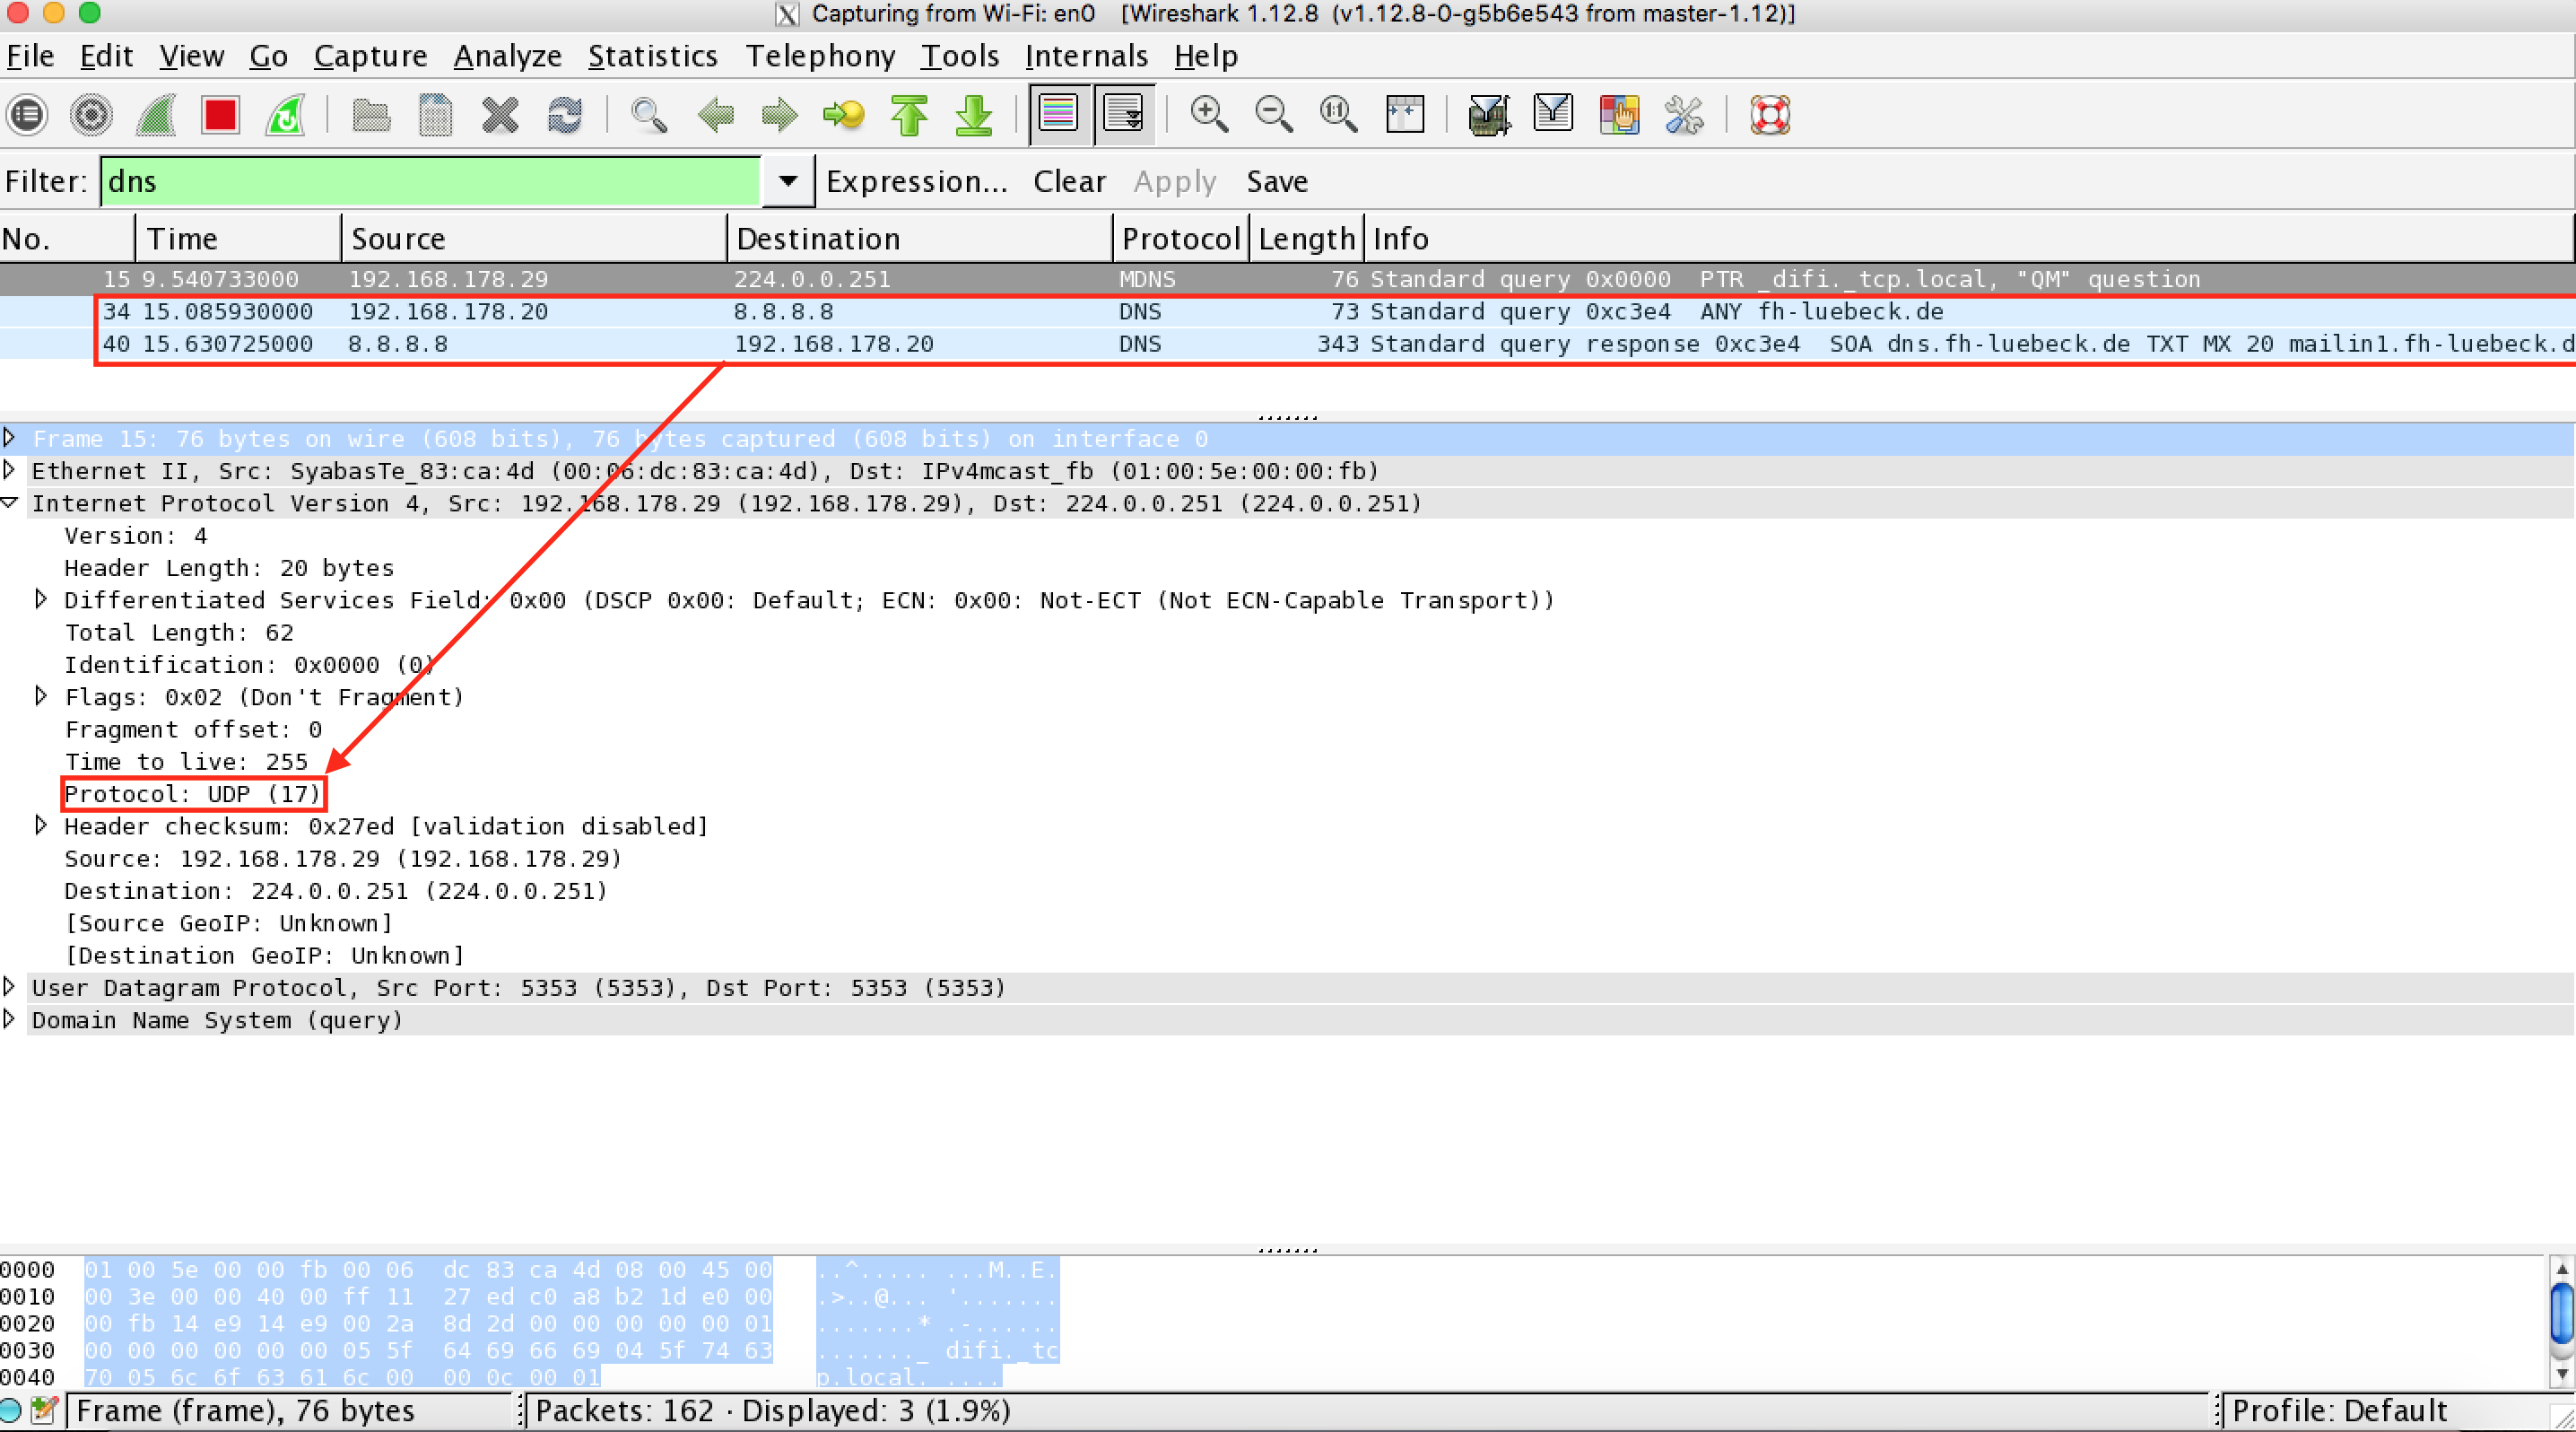
\includegraphics[width=15cm]{wirens8888}
    \label{fig:wirens8888}
  \end{figure}
  
  Hinter der DNS \textit{194.95.248.240} verbirgt sich die Website vom ''Deutschen Forschungsnetz'' (www.dfn.de).
  
    \begin{figure}
  \centering
    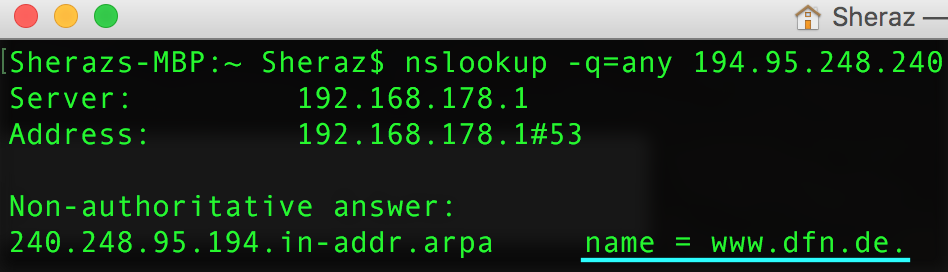
\includegraphics[width=10cm]{dfn}
    \label{fig:dfn}
  \end{figure}
  
  \begin{figure}
  \centering
    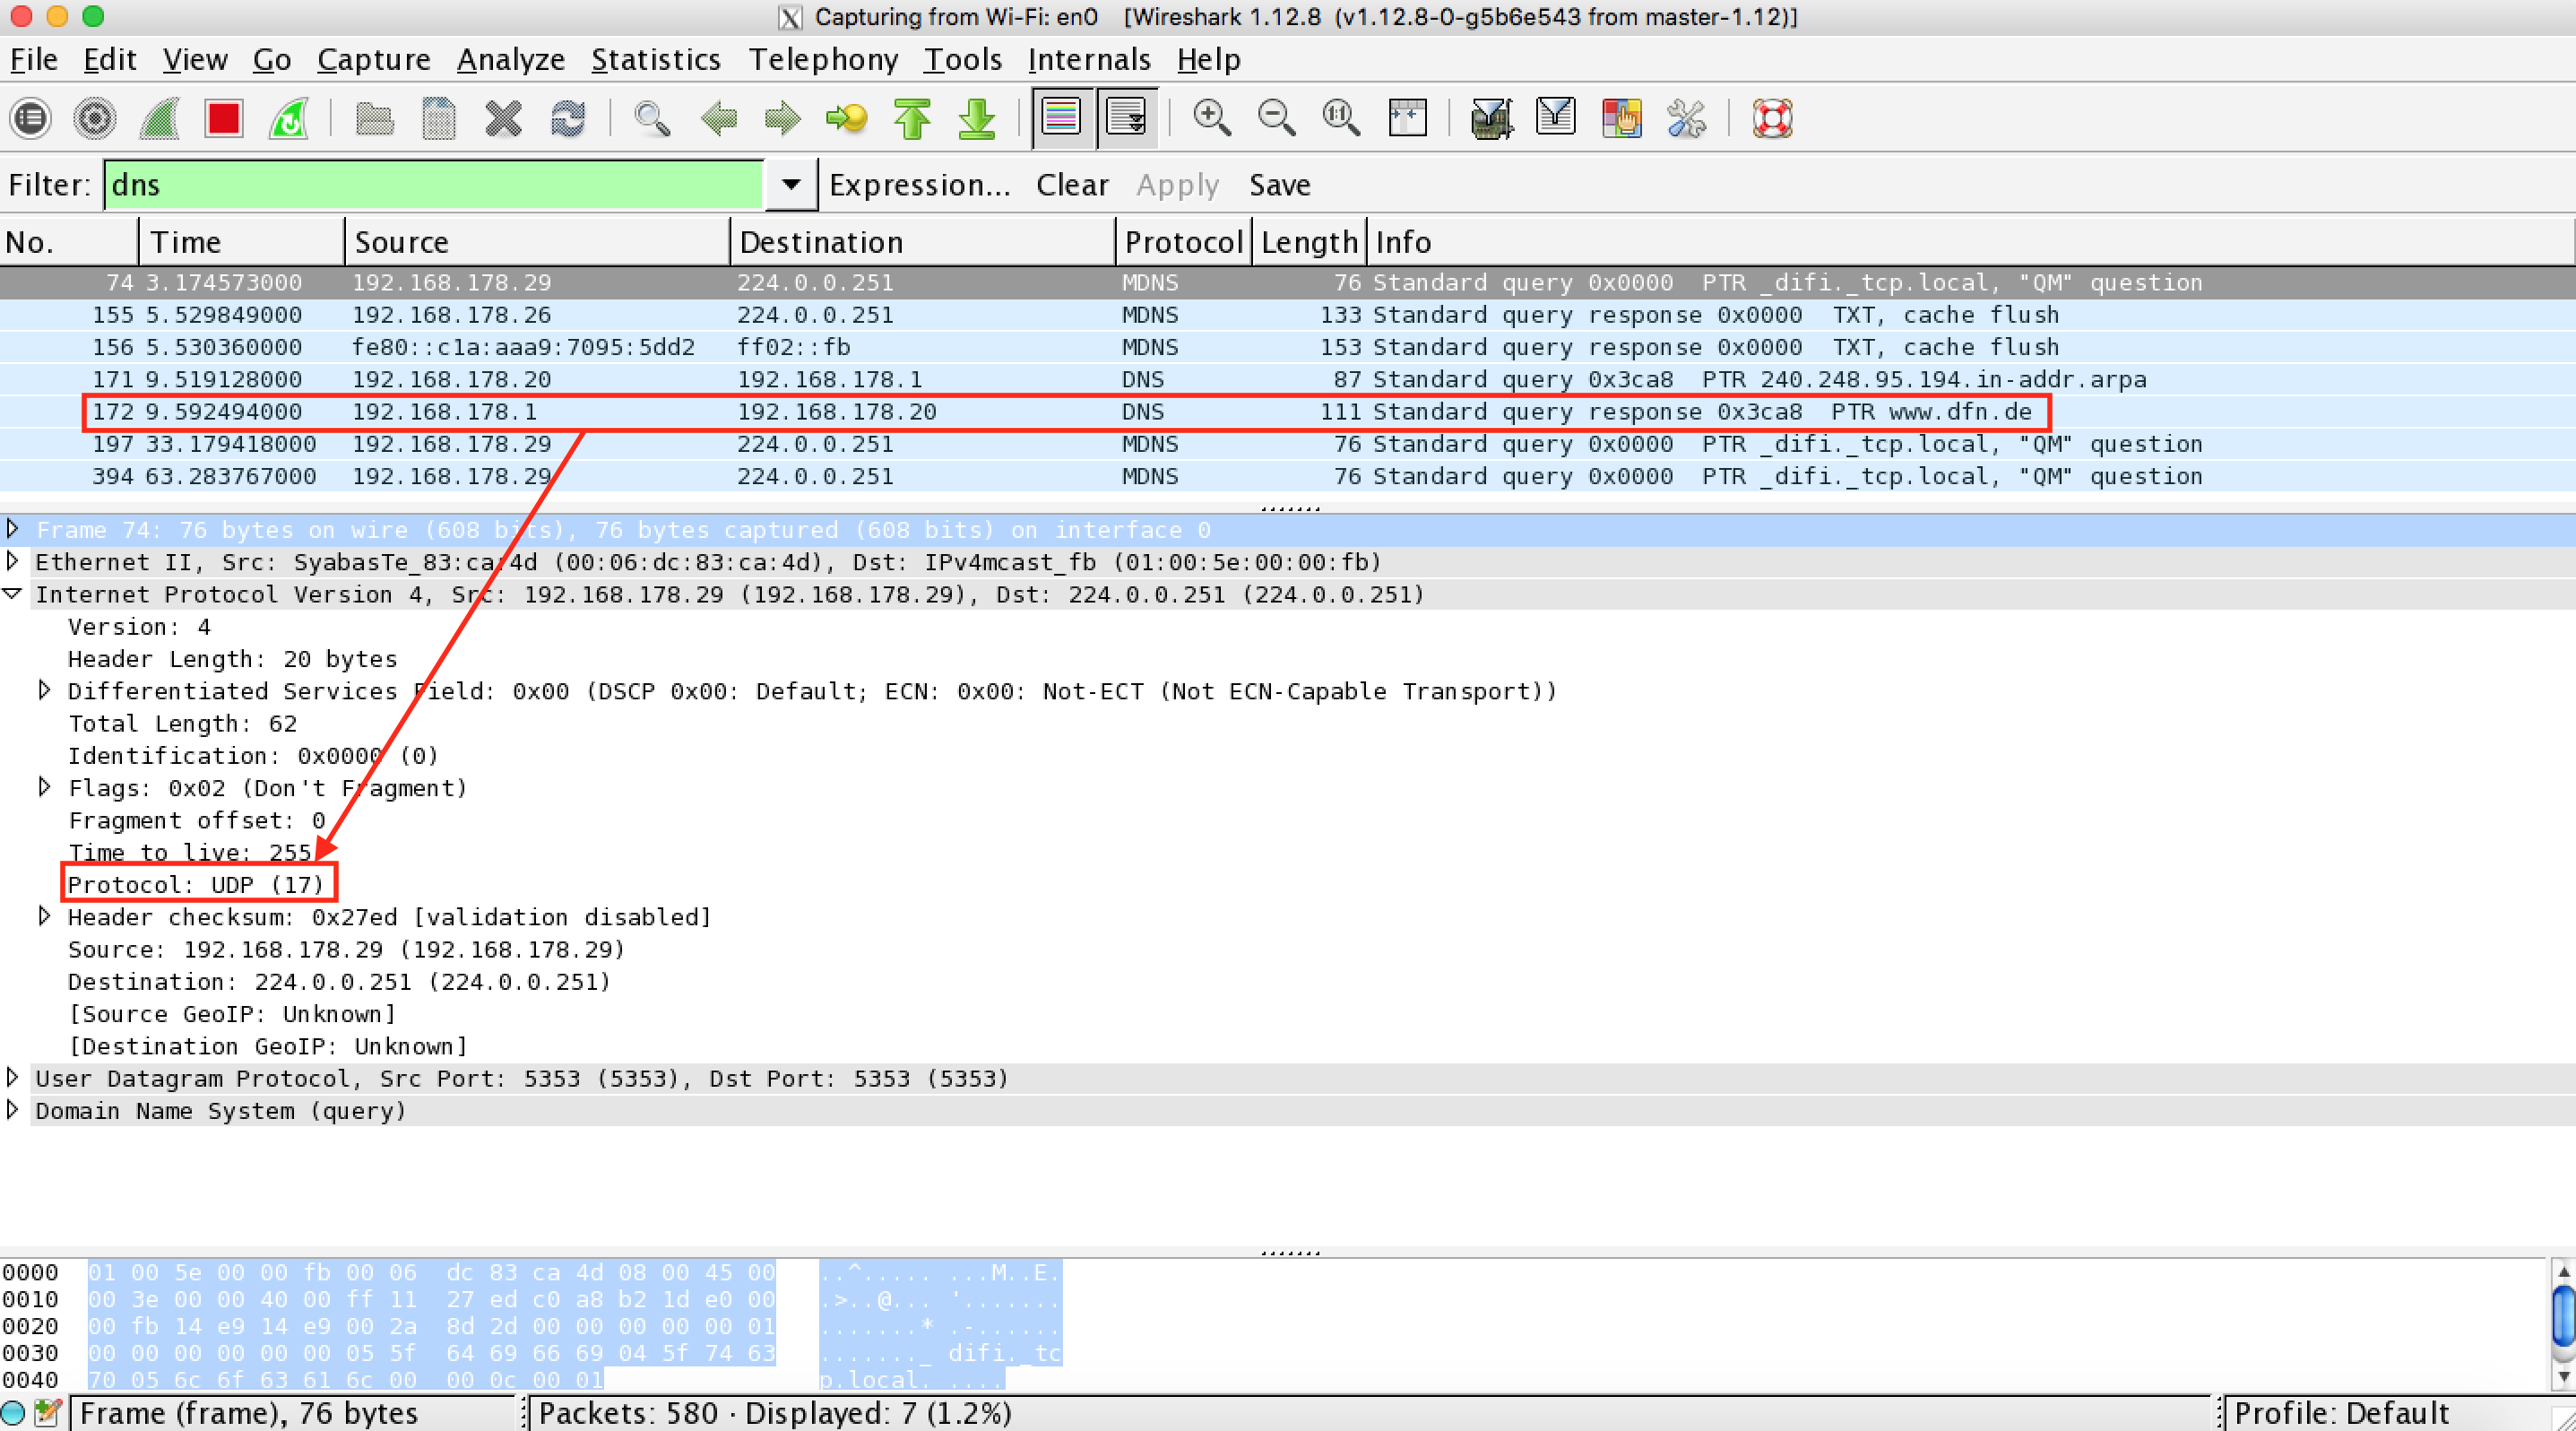
\includegraphics[width=15cm]{wiredfn}
    \label{fig:wiredfn}
  \end{figure}
  
  \subsection[Aufgabe 6 Aufbau von Websiten]{Aufbau von Websiten}
  
  Beim Aufruf der beiden Webseiten \emph{\textit{www.fh-luebeck.de}} und \emph{\textit{www.t-online.de}} mit aktivierten AddOns, wurden bei beiden mittels \textit{''IPvFox''} Hosts angezeigt die beim Aufruf der Webseiten als Ressourcen mit geladen wurden. Die Liste der Hosts von t-online.de war um ein dreifaches größer als der von fh-luebeck. 
  
  Nach und nach werden weitere Skripte mit \textit{''NoScript''} erlaubt/zugelassen, wobei auf beiden Websiten nun einige Hosts mehr geladen werden. Außerdem haben wir mit \textit{''Ghostery''} beide Websiten auf Tracker (Tracker dienen zur Analyse des Surfverhaltens eines Nutzers) untersucht. Auf t-online wurden vierzehn Tracker gefunden, wobei auf fh-luebeck erstaunlicherweise nur ein Tracker gefunden wurde.
  
  \subsection[Aufgabe 7 Laden von Websiten]{Laden von Websiten}
  
  Bei erneutem Laden der beiden Website, dieses mal mit gestartetem AddOn \textit{''Firebug''}, konnte festgestellt werden, dass es einige Inhalte oder Bilder gibt die t-online oder die fh-luebeck möglichst schnell bzw als erstes geladen haben möchte. 
  
  \begin{figure}
    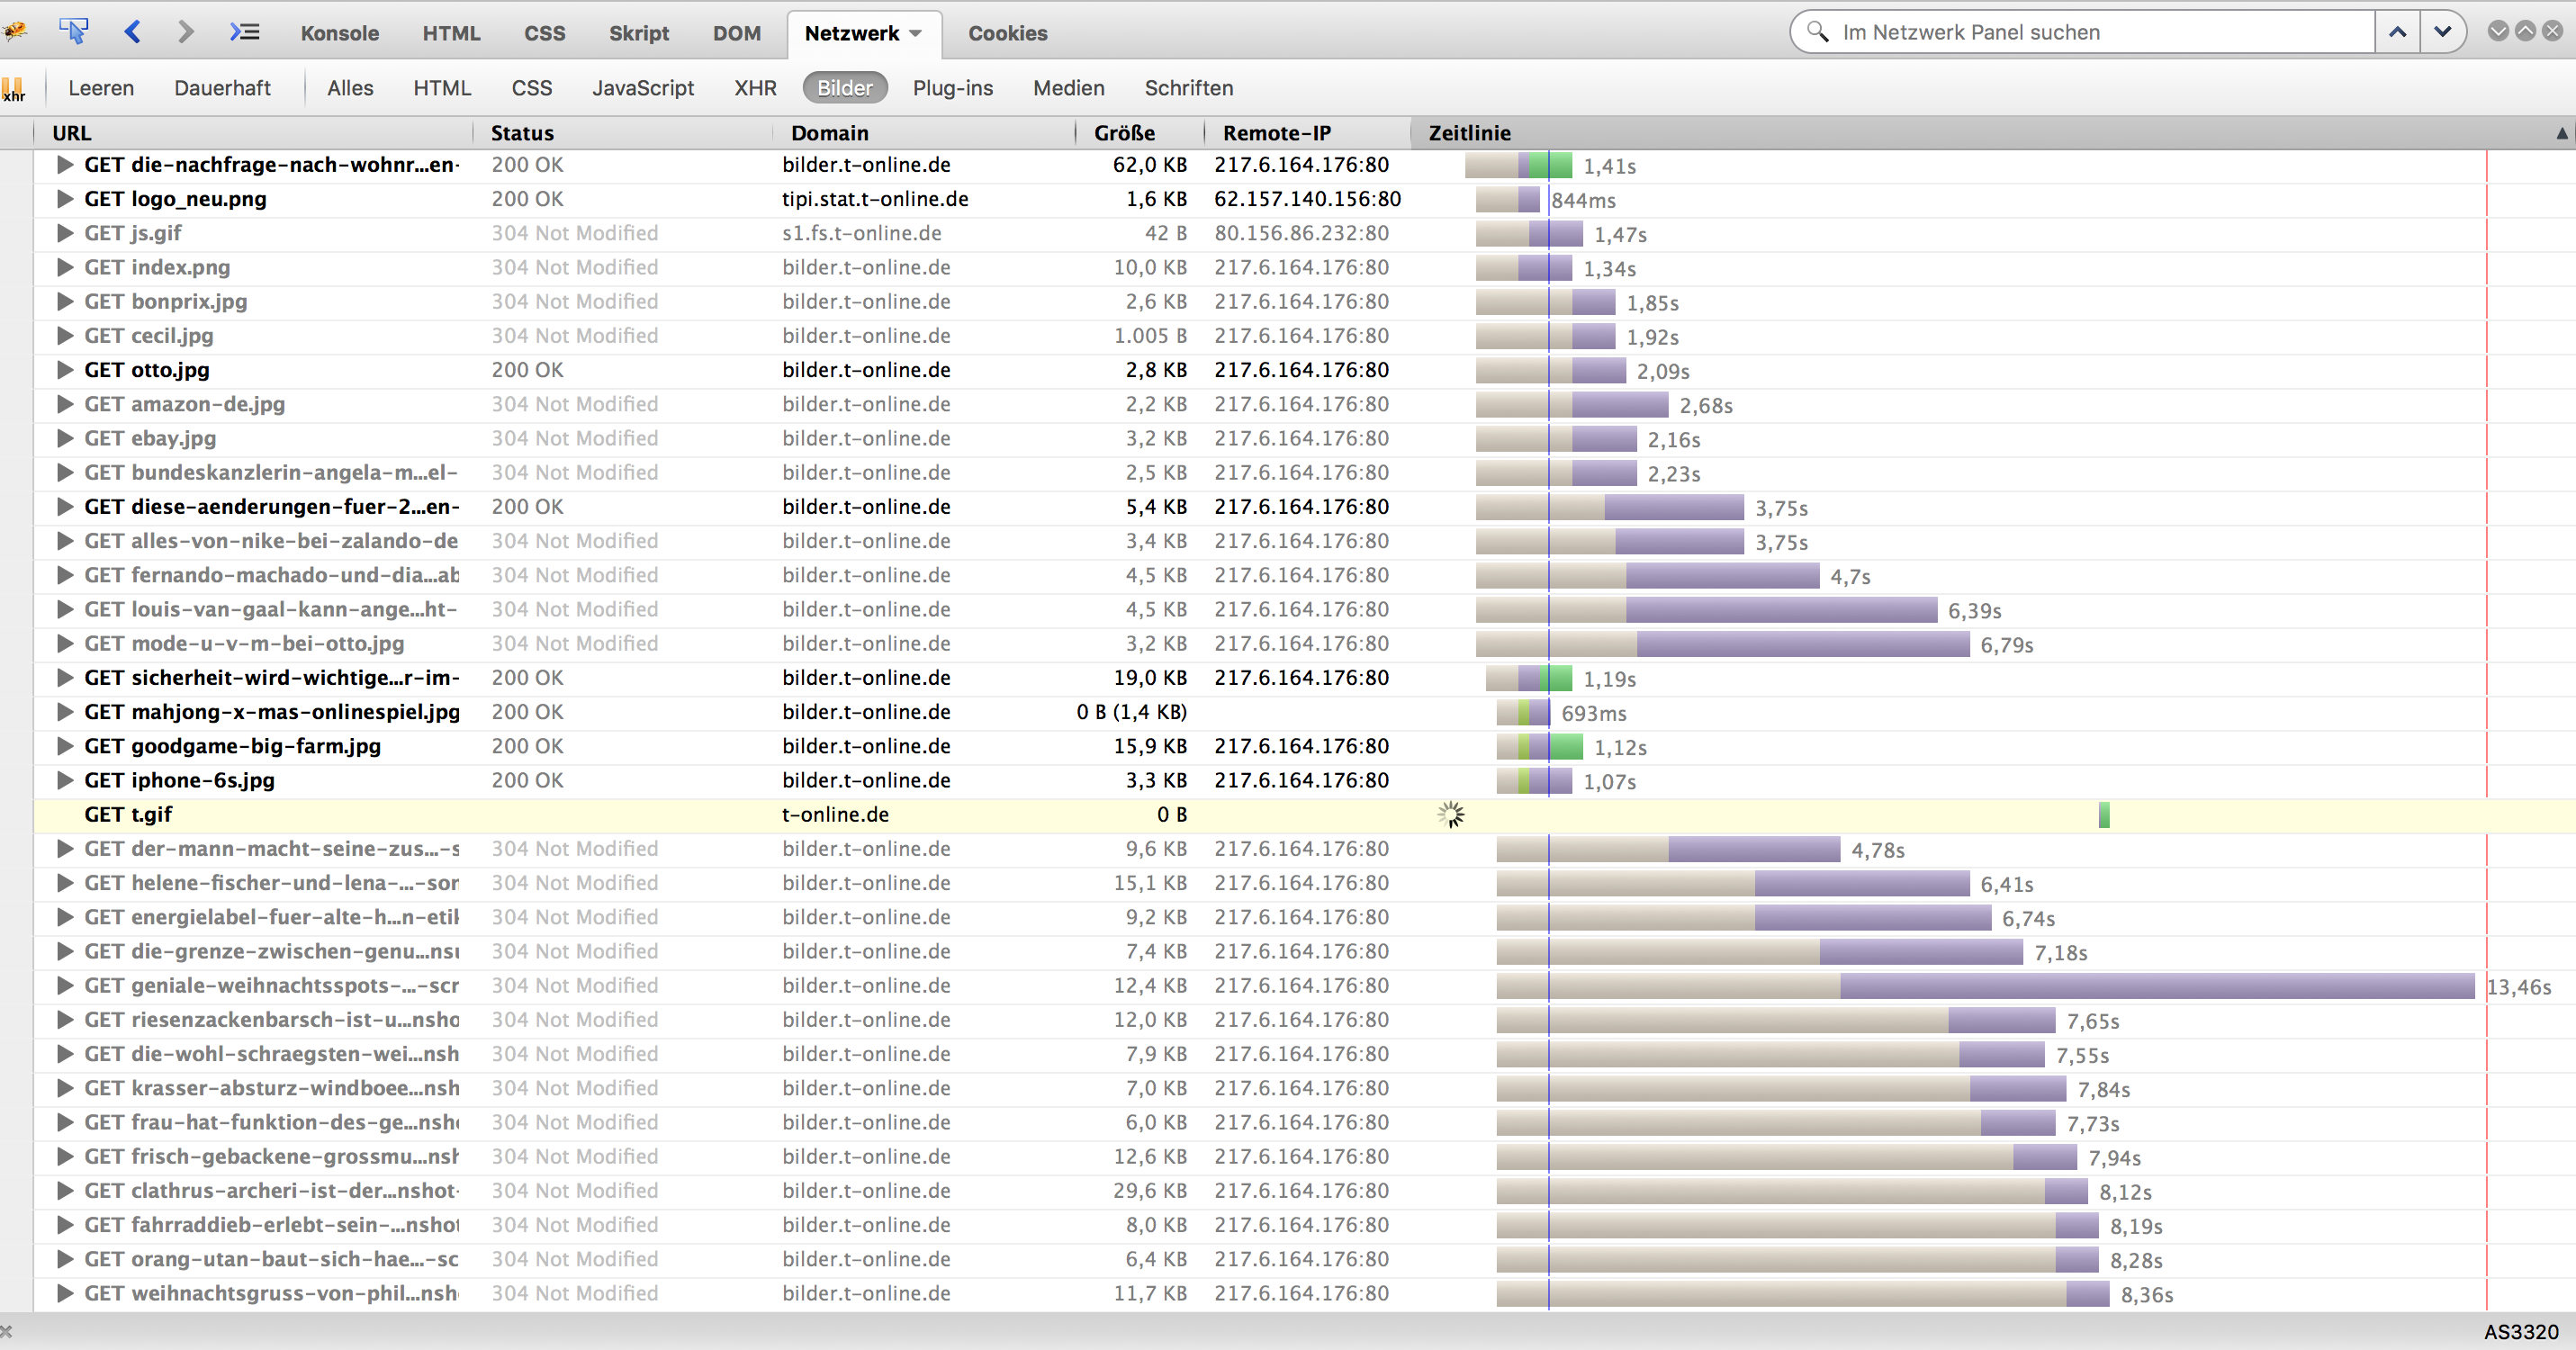
\includegraphics[width=15cm]{tonline}
    \label{fig:tonline}
  \end{figure}
  
  \begin{figure}
    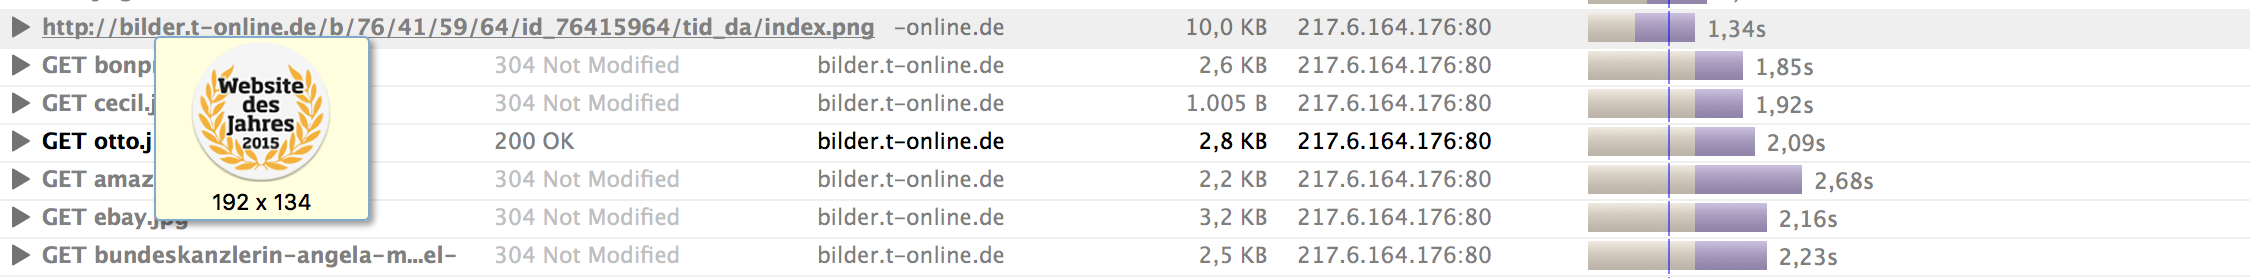
\includegraphics[width=15cm]{tonlinewin}
    \caption{T-Online Website des Jahres 2015}
    \label{fig:tonlinewin}
  \end{figure}
  
  Wie man in der Abbildung \ref{fig:tonlinewin} sehen kann, möchte T-Online natürlich dieses Bild vorher laden als, ein Icon auf der unteren Hälfte der Website.
  Außerdem fällt auf das nachdem die für t-online ''wichtigen'' Inhalte/Bilder geladen wurden, die Website anfängt Inhalte/Bilder der Werbeagenturen wie (Otto, Bonprix, Ebay, Amazon, etc) zu laden. 
  
  Ähnliches Prinzip finden wir bei der Website \emph{\textit{www.fh-luebeck.de}}, hier werden auch erst das Logo und dann die Bilder für die Kategorie \textit{''Aktuelles der Fachhochschule Lübeck''} geladen. Angesichts dieser Fakten kann man davon ausgehen das beide Websiten beim laden Ihrer Inhalte/Bilder Prioriäten setzen, in welcher Reihenfolge was geladen werden soll.
  
  \begin{figure}
  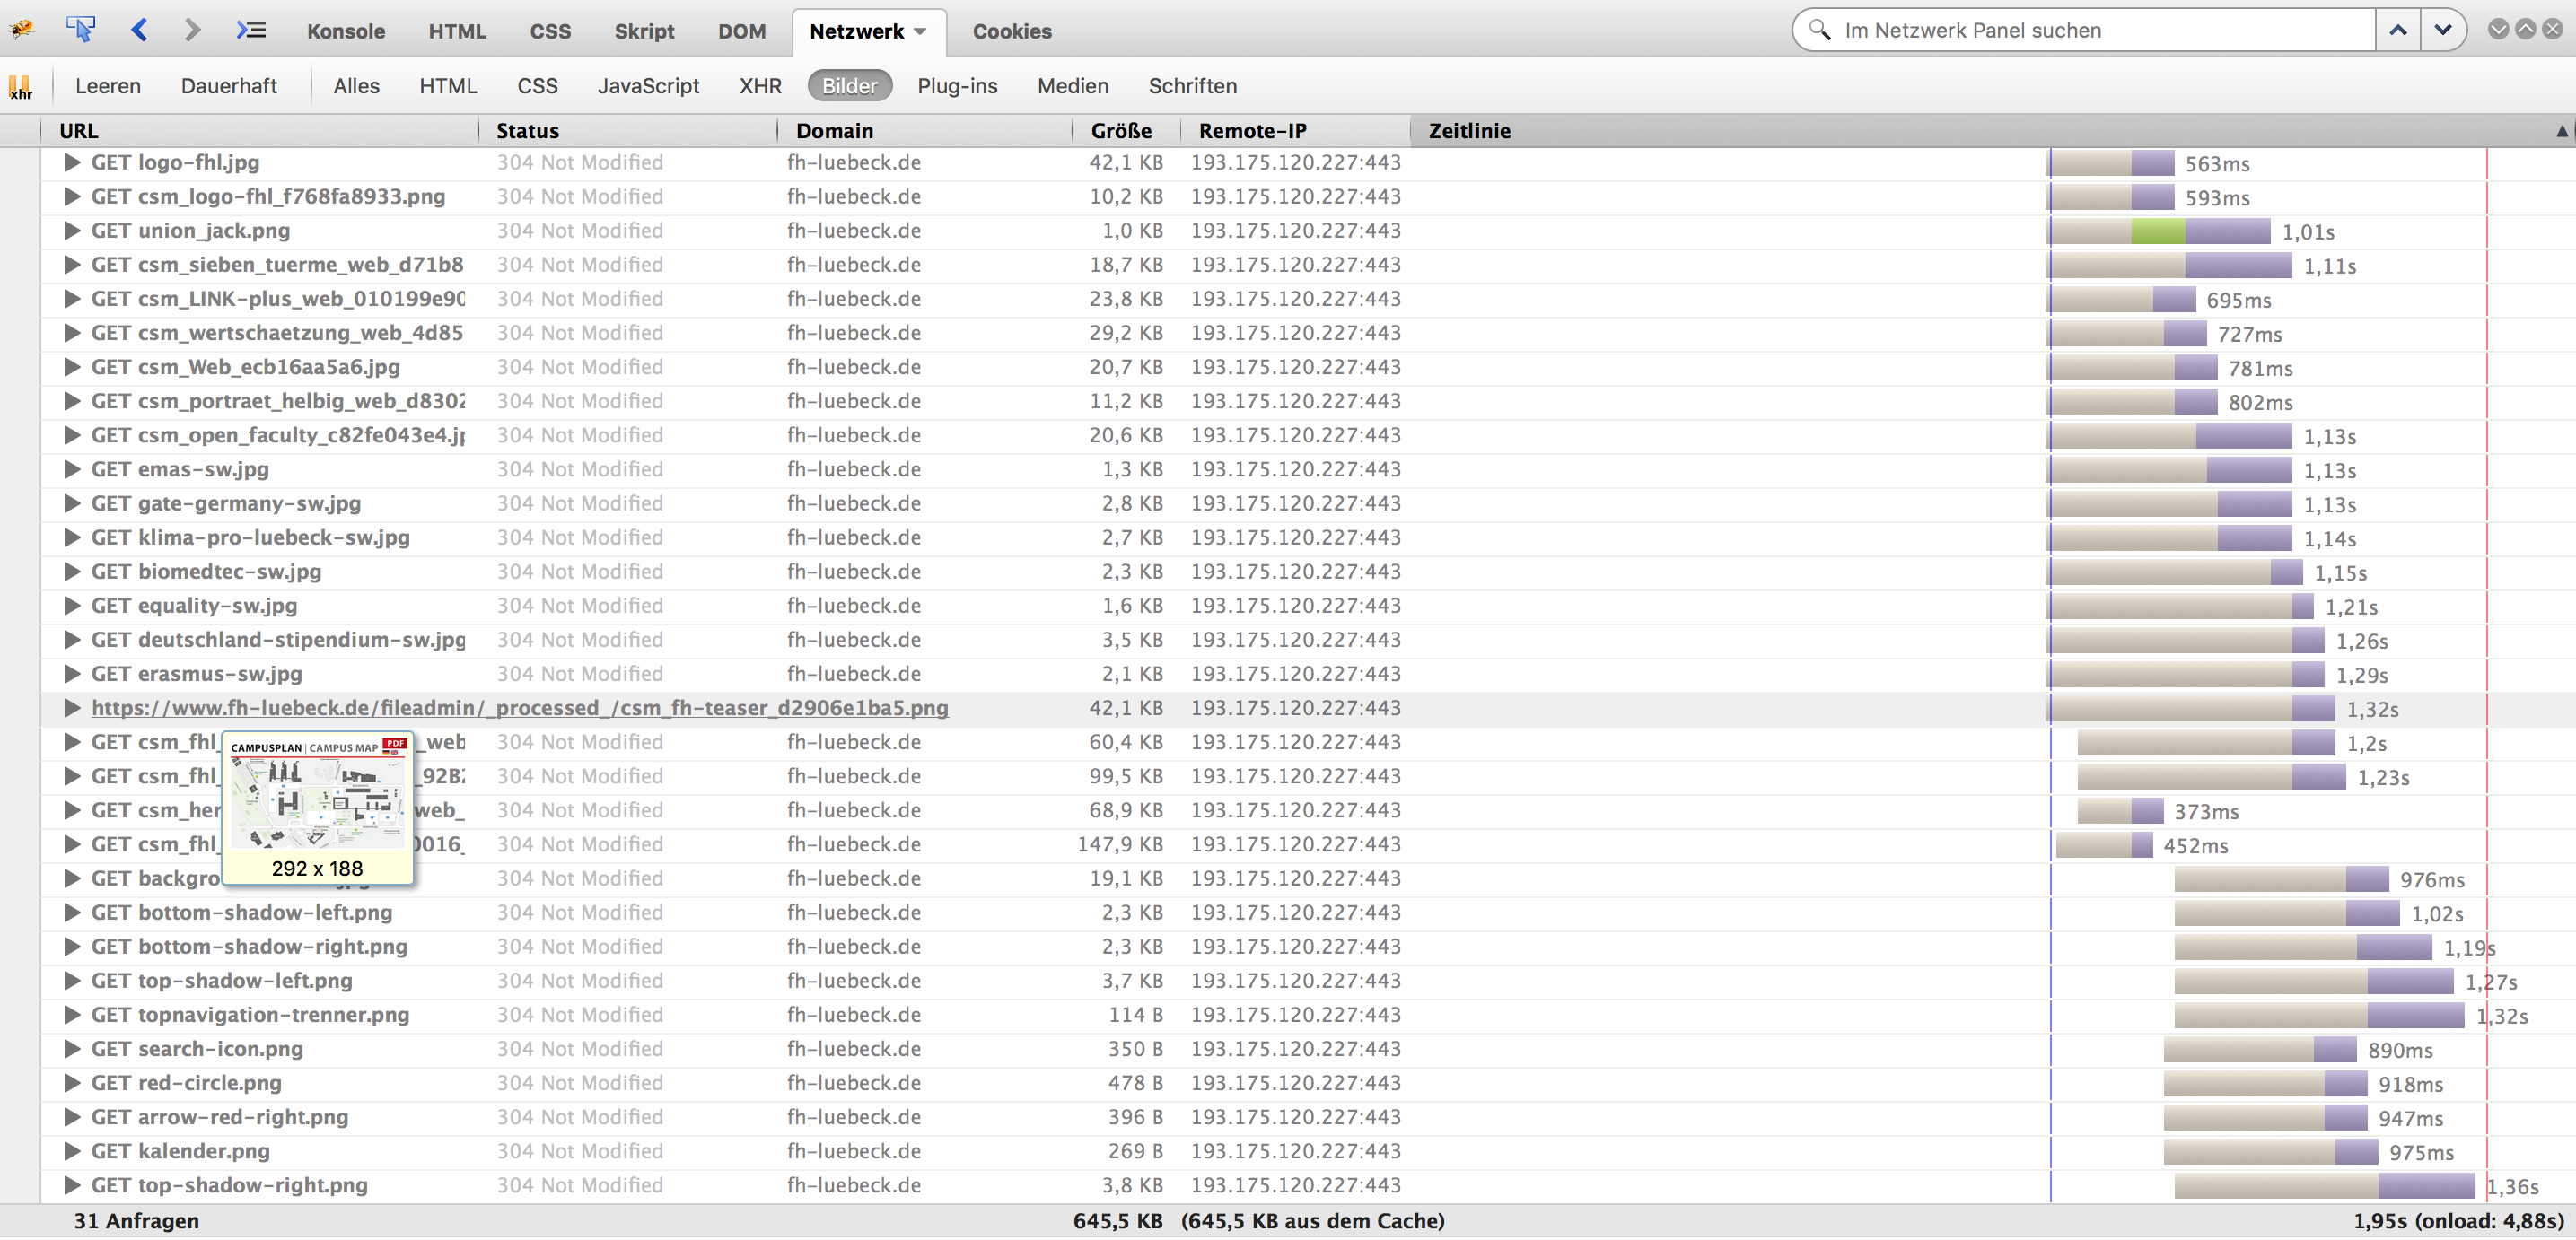
\includegraphics[width=15cm]{fhluebeck}
  \label{fig:fhluebeck}
  \end{figure}
  
  \subsection[Aufgabe 8 SSL/TLS im Browser]{SSL/TLS im Browser}
  
  \textbf{HIER DIE ANTWORT VON SVEN NOCH ABWARTEN WAS ER ZU DEM VERGLEICH DER BILDER SAGT}
  
  Mit der Website von \emph{\textit{https://cc.dcsec.uni-hannover.de/}} wurden die Browser Firefox und Safari getestet. 
  Dabei konnte man eindeutig feststellen
  Außerdem können wir in die Suchleiste von Firefox \textit{about:config} eingeben und so manuell SSL/TLS Einstellungen vornehmen.
  
  \subsection[Aufgabe 9 SSL/TLS beim Server]{SSL/TLS beim Server}
  
  Mit Hilfe der SSL Tools wurden die Seiten \emph{\textit{www.signin.ebay.de}} und \emph{\textit{www.banking.haspa.de}} untersucht. Hierbei lieferten beide das Ergebnis ''A-'', welches ein sehr unerwartetes und entäuschendes Ergebnis ist.
  Man hatte bei beiden Websiten ein Ergebnis von ''A++'' erwartet, da beide eine Möglichkeit für Online Transaktionen sind. Die Protkolle auf solchen Seiten sollten immer aktuell und im Schnitt ''A+'' haben.
  
  \begin{figure}
  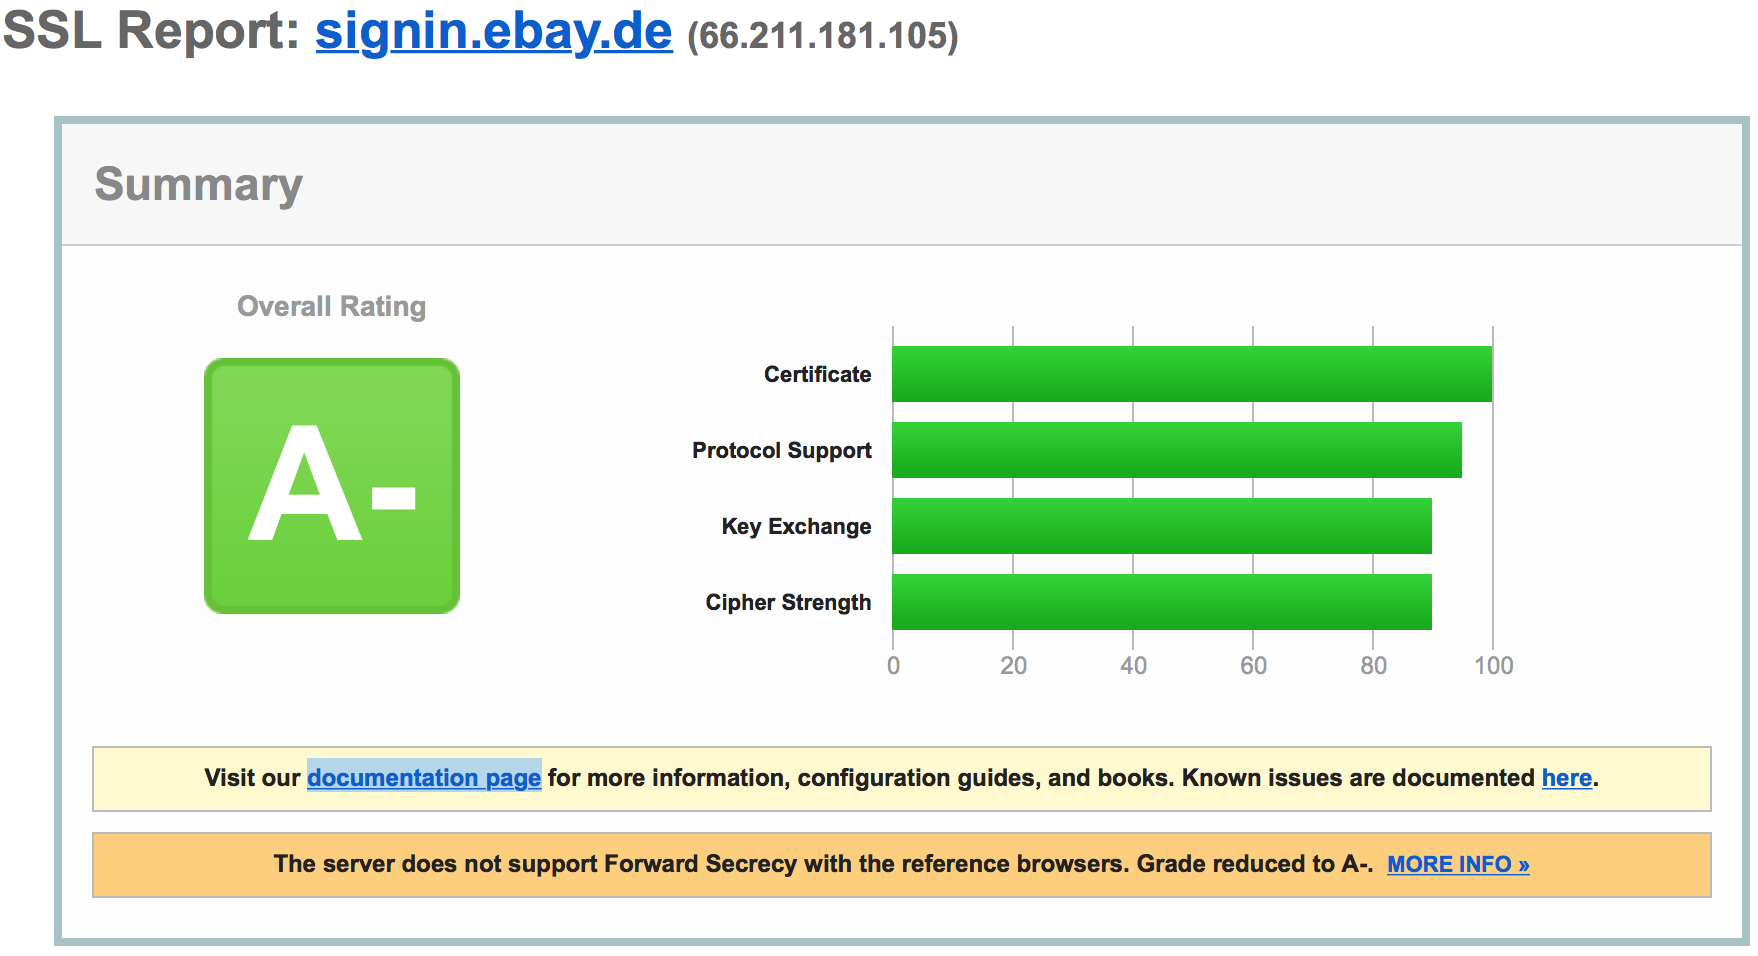
\includegraphics[width = 15 cm]{ebay}
  \label{fig : ebay}
  \end{figure}
  
  \begin{figure}
  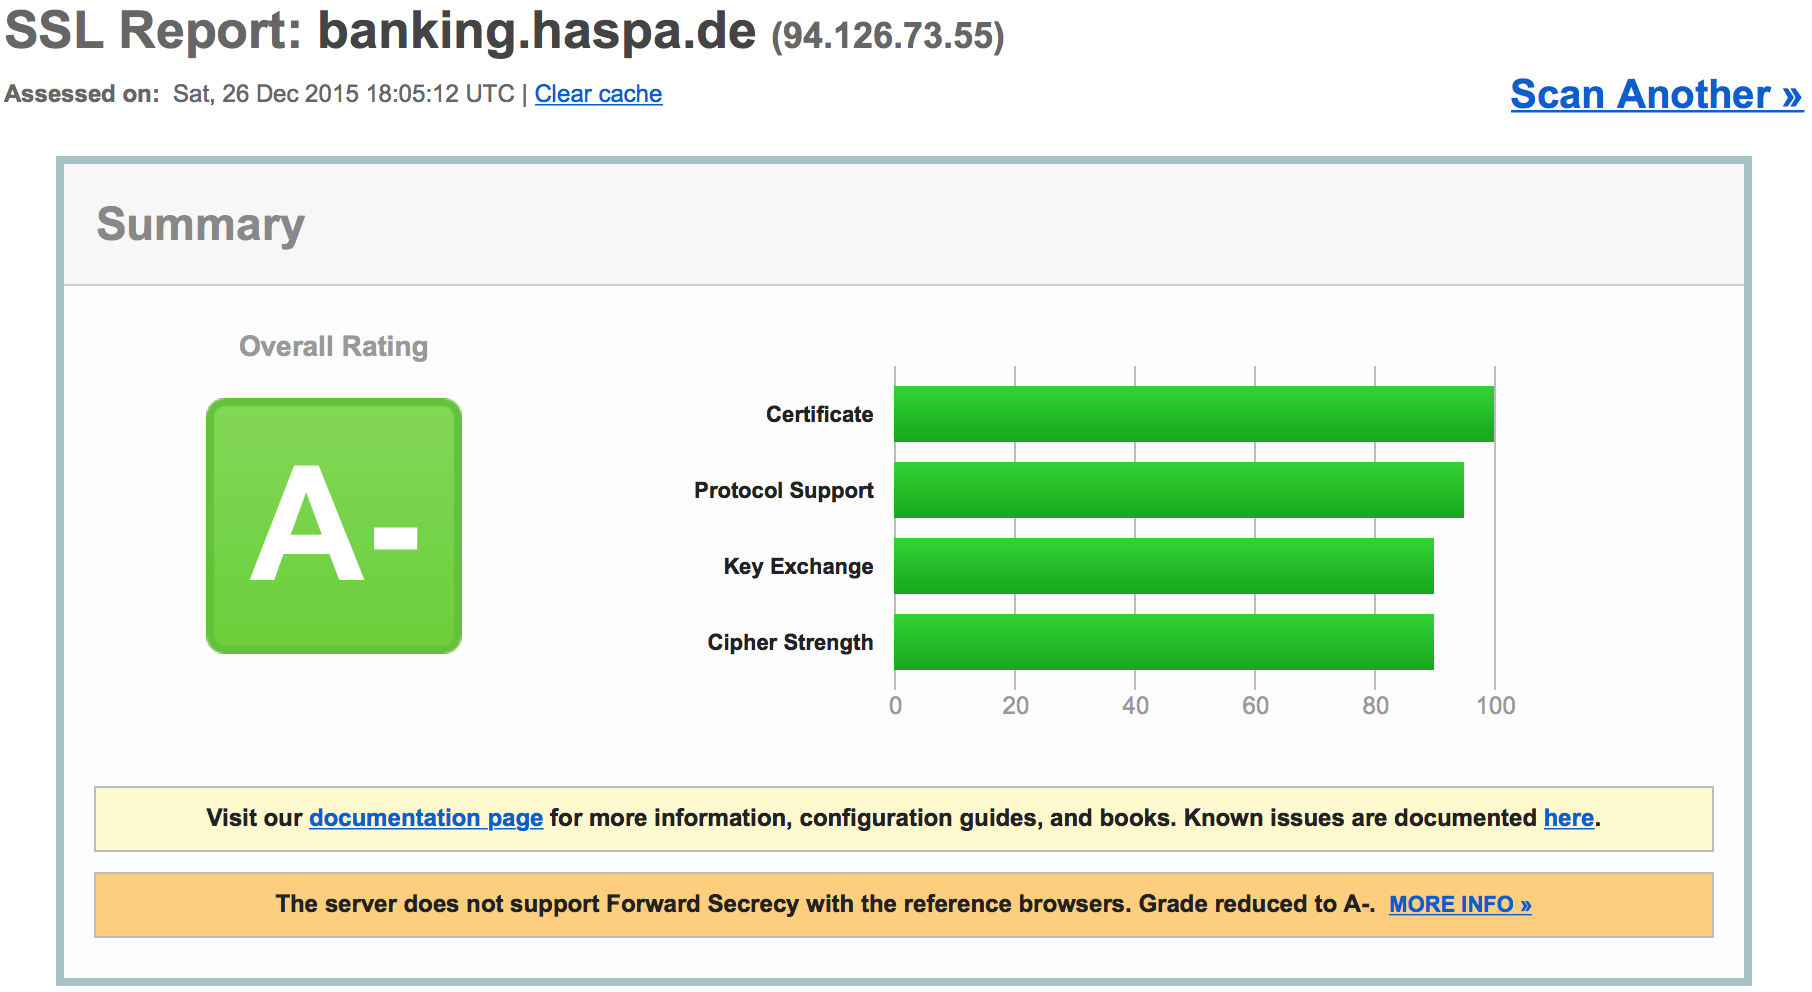
\includegraphics[width=15cm]{bank}
  \label{fig:bank}
  \end{figure}
  
  \subsection[Aufgabe 10 Auswertung von Cookies]{Auswertung von Cookies}
  
  Im Laufe des Praktikums haben sich sehr viele Cookies angesammelt, viele davon sind von Dirttanbiertern die man, wenn man sich davor mit Cookies nie befasst hat, nicht kennt. Es haben sich ca. 80 Cookies angesammelt. 
  Mit \textit{''Cookie Monster''} kann Einstellungen vornehmen wie einzelne Cookies zu erlauben oder alle/keine Cookies erlauben. Außerdem kann man noch sehen welcher Cookie von welcher Website ist.
  
  \subsection[Aufgabe 11 Diskussion AddOns]{Diskussion AddOns}
  
  \textbf{Firebug} ist kein gutes AddOn für Netzwerkspezialisten oder Entwickler, aber für einen ''normalen'' Anwender hat dieses AddOn wenig Sinn.\\ 
  \emph{Fazit:} Wir werden dieses AddOn weiterhin \textbf{nicht benutzen}.
  
  \textbf{No Script} ist ein sehr sinnvolles Tool, da es nicht nur Sicherheit mit sich bringt sondern auch noch die Leistung steigert. Da man durch dieses Tool sinnlose Werbungen und Scripte deaktivieren kann, läd die Website viel schneller. Jedoch kommt es ab und zu vor das man eine Website besucht und ein bestimmtes Skript verwenden will welches aber von dem Tool blockiert wird, dies is jedoch kein großes Problem, da man manuell Skripte temporär oder für immer für die Webiste erlauben kann. \\
  \emph{Fazit:} Da wir vor dem Praktikum schon dieses AddOn kannten und verwendet haben, werden wir es auch in der Zukunft weiterhin \textbf{benutzen}.
  
  \textbf{Ghostey} dient zum blockieren der Tracker und man hat immer den Überblick über die Tracker, da sie oben rechts auf dem Bildschirm beim laden der Website angezeigt werden.\\
  \emph{Fazit:} Wir kannten das AddOn vorher nicht und waren sehr beeindruckt und werden es in der Zukunft \textbf{benutzen}.
  
  \textbf{CookieMonster} lässt sich sehr einfach bedienen und man kann leicht Cookies ganz oder einzelnd erlauben und verbieten.\\
  \emph{Fazit:} Auch dieses AddOn war uns zuvor bekannt und wir werden es weiterhin \textbf{benutzen}.
  
  \textbf{DNSSec Validator} prüft ob eine Website mit DNSSec geschützt ist. Man muss einige Einstellungen vornehmen, bevor man dieses AddOn zum laufen bekommt.\\
  \emph{Fazit:} Da wir keinen sinnvollen Anwendungsfall im Alltag dafür finden, werden wir dieses AddOn \textbf{nicht benutzen}.
  
  
  \subsection[Aufgabe 12 Steganographie]{Steganographie}
  
  Im Bild war die Datei ... enthalten und man konnte mit dem bloßen keinen einzigen Unterschied zwischen den beiden Bildern finden.
  
  \textbf{SVEN NOCHMAL FRAGEN WELCHE DATEI DA RAUS KAM UND WAS MAN MIT DER HISTOGRAMM FUNKTION GESEHEN HAT}
       
%----------------------------------------------------------------------------------------------------------------------------
  \newpage
\section[Versuch 4 Switch]{Switch}

  \subsection[Aufgabe 3 MAC-Adresse]{MAC-Adresse}
  
  Die MAC-Adresse wurde mit dem Befehl \textit{ipconfig/all} unter dem Punkt ''Physikalische Adresse'' gefunden \ref{fig:ipconfigall}. Mittels der Website \\ 
  \emph{\textit{ http://standards.ieee.org/regauth/oui/index.shtml}} wurde der in Abbildung \ref{fig:macaddr} abgebildete Hersteller gefunden.  

  \begin{figure}
    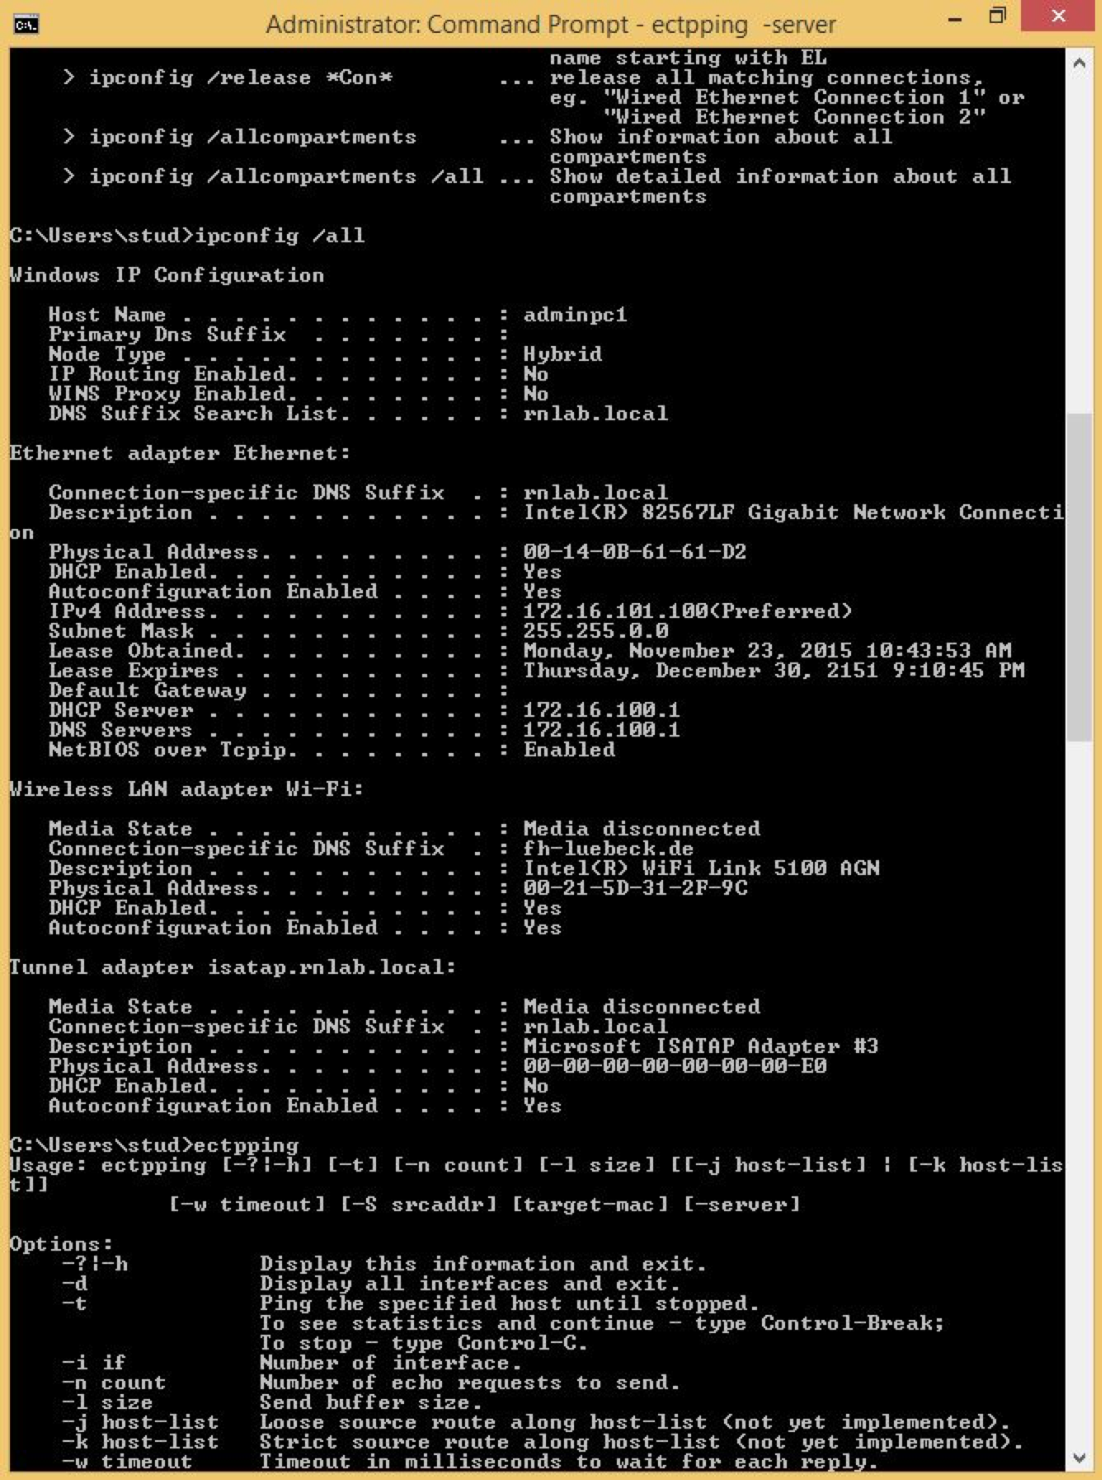
\includegraphics[width=10cm]{ipconfigall}
    \label{fig:ipconfigall}
  \end{figure}
     
  
  \begin{figure}
    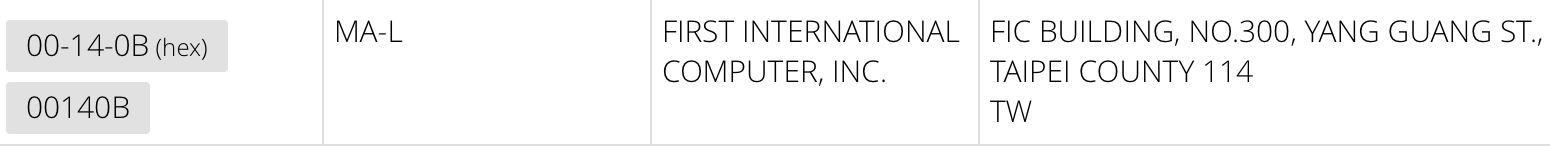
\includegraphics[width =10cm]{macaddr}
    \caption{Hersteller}
    \label{fig:macaddr}
  \end{figure}
  
  \subsection[Aufgabe 4 Beobachtungen im Netz]{Beobachtungen im Netz}
  
  \renewcommand{\labelenumi}{\alph{enumi})}
  \begin{enumerate}
  \item
  Die folgenden Befehle wurden auf dem Admin-PC und dem Lab-PC, wie man in der Abbildung sehen kann erfolgreich durchgeführt und mit Wireshark aufgezeichnet.\\
  \textbf{ectpping - mac destination} (Admin-PC)\\
  \textbf{ectpping - server} (Lab-PC)
  
  \begin{figure}
    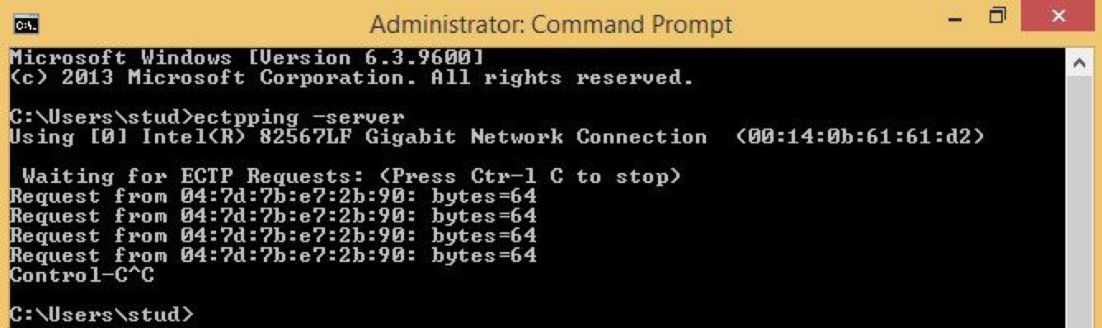
\includegraphics[width=10cm]{ectppingserver}
    \label{fig:ectppingserver}
  \end{figure}
  
  \item
  Um nur die Rahmen der Kommunikation von ectpping herauszufinden, kann man nach dem Protokoll ''LOOP'' filtern. In diesem Beispiel wird der Ethernet II Rahmentyp verwendet, welches man anhand der Abbildung \ref{fig:loops} ablesen kann.
  
  \begin{figure}
    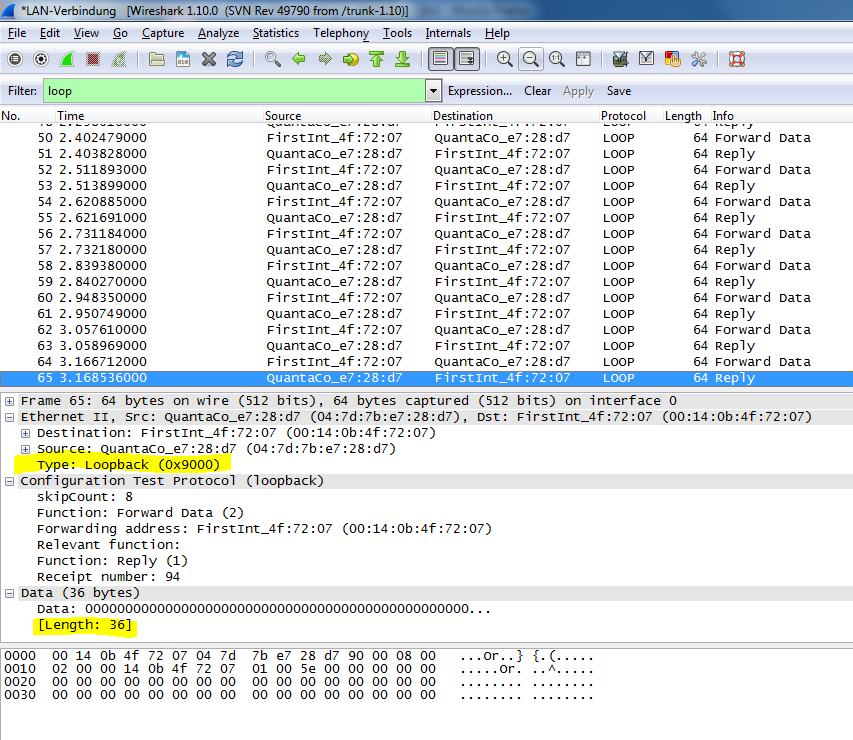
\includegraphics[width=10cm]{loops}
    \label{fig:loops}
  \end{figure}
  
  \item
  Durch das umstecken der Netzwerkkabel entsteht eine Endschlosschleife. Eine Netzwerküberlastung wird sofort sichtbar, da es keine Regelungen für redundante Pakete gibt. Als Lösung könnte man wie in Versuch 2 schon besprochen Sequenznummern einführen.
  
  \item
 \textbf{KEINE NOTIZEN DAZU  SVEN ODER ANDERE GRUPPE FRAGEN}
 \end{enumerate}
 \subsection[Aufgabe 5 Spanning Tree Protocol]{Spanning Tree Protocol}
 
  \renewcommand{\labelenumi}{\alph{enumi})}
  \begin{enumerate}
  \item
  Erst wurde die Nachricht \textit{No spanning tree Instance exists} zurückgegeben. Nachdem das Spanning Tree Protocol mit den gegebenen Befehlen eingeschaltet wurde, wurde eine Tabelle zurückgeliefert, welche alle Schnittstellen mit Informationen über ihre Kosten und andere enthielt. 
  
  \begin{figure}
    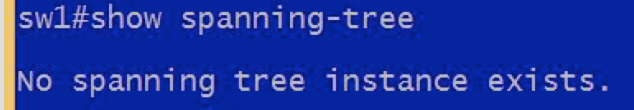
\includegraphics[width=10cm]{showspan}
    \label{fig:showspan}
  \end{figure}
  
  \begin{figure}
    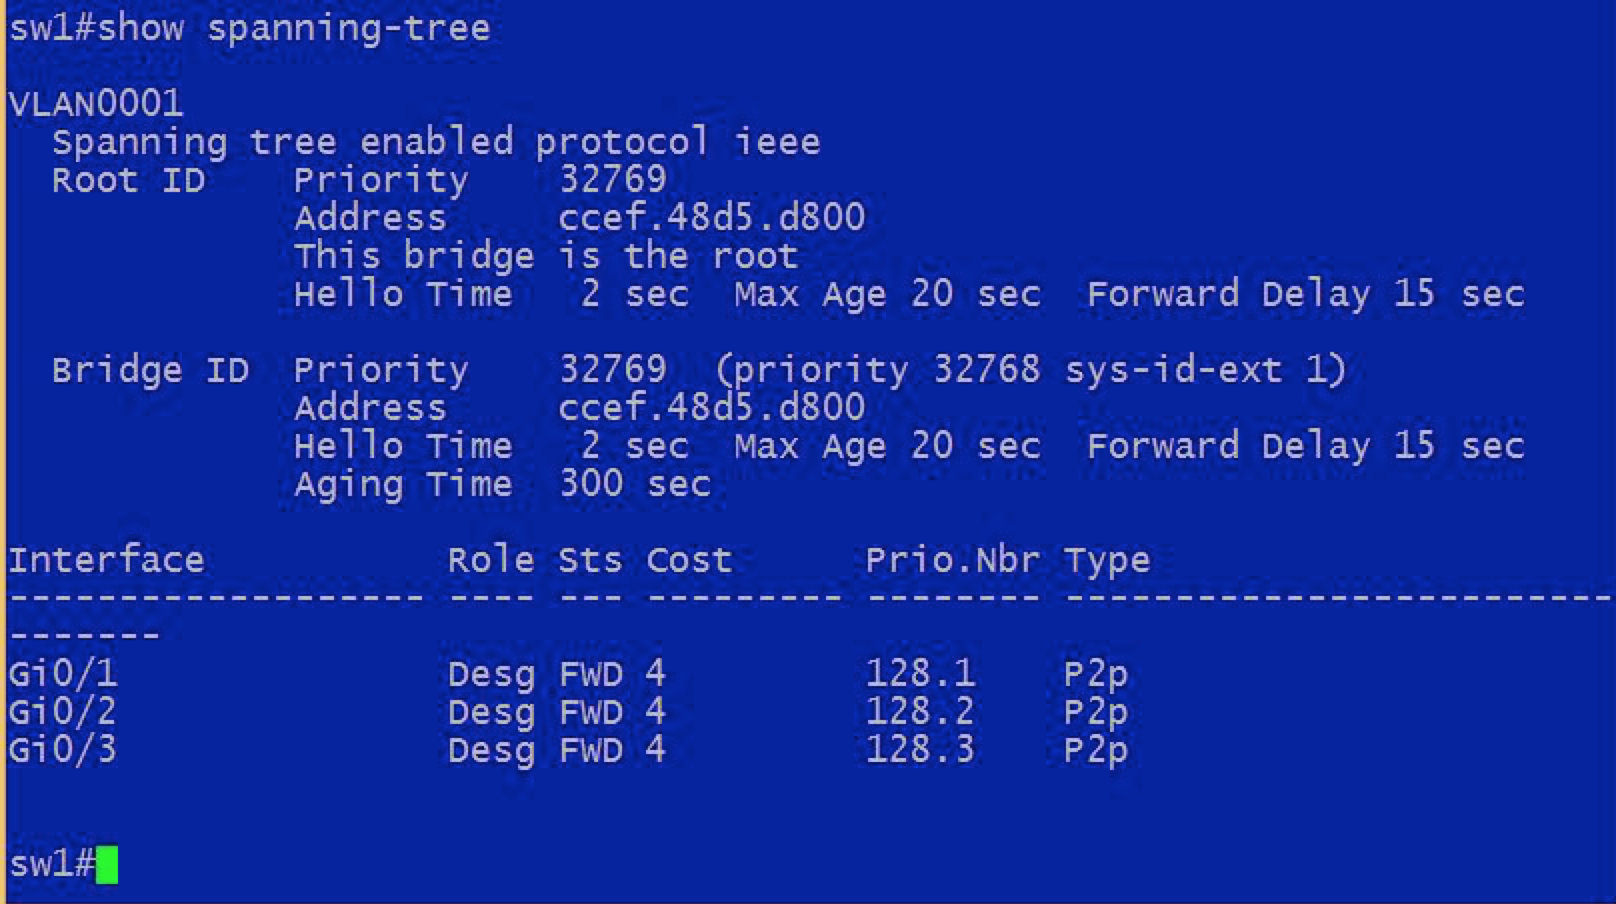
\includegraphics[width=15cm]{spanningtree}
    \label{fig:spanningtree}
  \end{figure}
  
  \item
  Um Schleifzustände zu vermeiden versetzt der STP die Ports, die zusammen den Spanning Tree bilden, in fünf verschiedene Portzustände. Diese Portzustände werden mittels Timer für jeden Portzustand berechnet. In der Tabelle unten sieht man die fünf Zustände die Ports annehmen können. \footnote{www.airnet.de}
  
  \begin{table}
  \begin{tabular}{|l|l}
      \textbf{Portzustand} & \textbf{Beschreibung} \\ \hline
		 Disabled     & Administrativer shutdown \\
		 Listening    & Horchen auf BPDU-Pakete oder versenden von BPDU-Paketen \\
		 Learning     & Listening-Funktiond und lernen von Quell-MAC-Adressen \\
		 Forwarding & Listening- und Learning-Funktion und weiterleiten von Datenframes\\
        Blockeing    & Horchen auf BPDU-Pakete
    \end{tabular}
     \caption{Prozesstabelle (BPDU-Pakete sind spezielle Pakete die Switches senden können)}
    \end{table}
    
    Das STP findet redundante Kommunikationswege heraus und ändert die ganze Netzwerktopologie in eine Baumtopologie, die keine Schleifen besitzt. Die Kosten zur Root Bridge sind vier welches man aus der Abbildung \ref{fig:spanningtree} entnehmen kann.
    
    \item
    Das Team, welches das Kabel zum zentralen Switch entfernt, erhält höhere Kosten. Der Grund dafür ist, das dieser sich nun erst über einen anderen Switch verbinden muss um eine Verbindung zum Switch 0 herzustellen.
    
    \item
    \textbf{IST BEI UNS HIER EINE SCHLEIFE ENTSTANDEN ODER KAM HIER DASSELBE RAUS WIE ICH ES SCHON IN AUFGABE 5 b ERWÄHNT HABE ?}
    
    \item
    Typische Informationen vom STP sind:
    
    \begin{itemize}
      \item MAX Age
      \item Hello Time
      \item Forward Delay
    \end{itemize}
     Wobei die STP-Rahmen folgede Schichten beinhalten: 
     
 	 \textbf{ICH HABE KEINE NOTIZEN ZU DEN RAHMEN (war damit gemeint das mit längen und typ feld ? oder ist damit gemeint welche Tabs angezeigt werden ? das kann man aus den Bildern von Wireshark entnehmen) SONST WIEDER JEMANDEN FRAGEN }
  \end{enumerate}

   \subsection[Aufgabe 6 Lernen von Adressen für die MAC-Adresstabelle]{Lernen von Adressen für die MAC-Adresstabelle}
   
  \renewcommand{\labelenumi}{\alph{enumi})}
  \begin{enumerate}
    \item
    In einem Intervall von 300 s sind erneuerungen der Adressen notwendig, wie man in der Abbildung unten sehen kann.
    
    \begin{figure}
    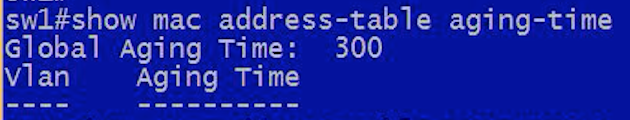
\includegraphics[width=10cm]{aging}
    \label{fig:aging}
    \end{figure}
  
  \item
  Die Einträge waren in sehr kurzer Zeit wieder in der Tabelle eingetragen. Da wir in einem vorhandenem Netzwerk sind und die Switch (wie wir in der Vorlesung gelernt haben) selbstlernend (self-learning) ist, speichert diese Einträge selbstständig in die Tabelle. Die Einträge beinhalten folgende Informationen, die MAC-Adresse, die aktuelle Zeit und die Schnittstelle über die der Rahmen eingetroffen ist.
  
  \item
  Durch den Broadcast an andere unbekannte Ziele, hat die Adresstabell weitere ''DYNAMIC'' Einträge dazu bekommen, weil der Switch diese Adressen schnell dazu gelernt hat.
  
  \item
  Während beim fortlaufenden ectpping der Port abgezogen wurde, kam die Meldung \textit{''Request Timed out''} für ca. 10 s, danach jedoch ging es ''normal'' weiter. Wie schon in den Aufgaben davor besprochen lässt sich dieses Verhalten durch das selbstlernen des Switches erklären. Beim Umstecken der Ports hat Wireshark angezeigt das, dass STP aktiviert wurde.
  
  \begin{figure}
  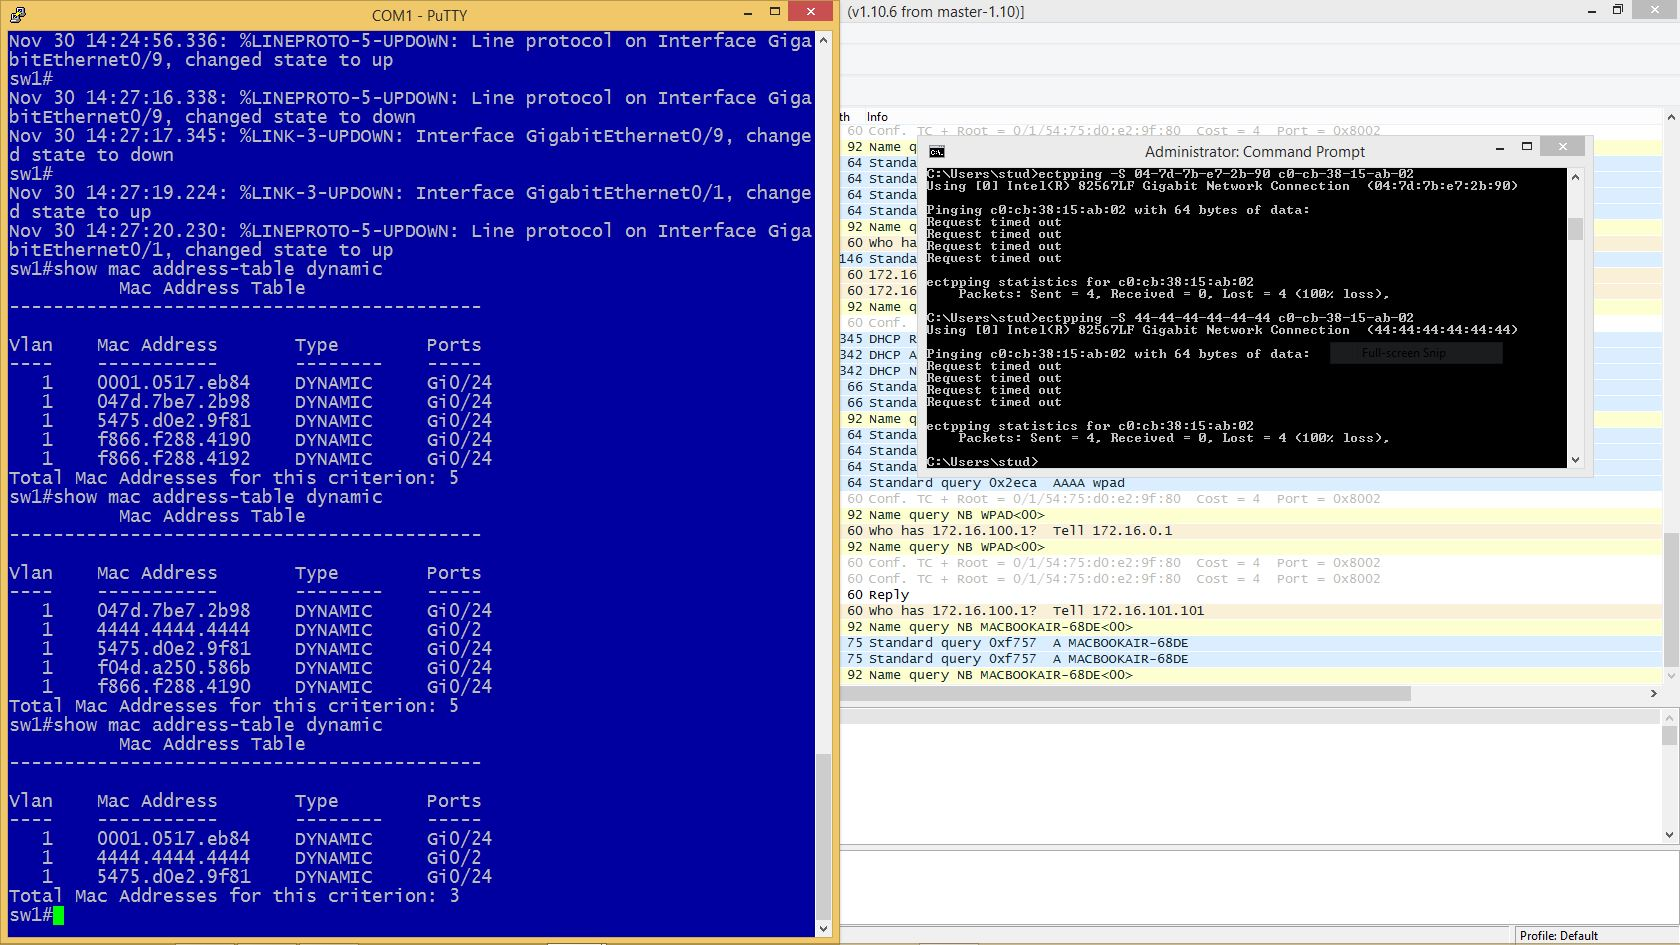
\includegraphics[width=10cm]{switch}
  \label{fig:switch}
  \end{figure}
  
  \item
  Die Quelladresse lässt sich sehr leicht manipulieren ist jedoch zwiespaltig zu beurteilen. Aus Sicht des Senders ist eine gute Möglichkeit sich als jemand anderes auszugeben, doch aus Sicht des Empfängers ist es sehr gefährlich, da wenn als Sicherheitsmaßnahme nur die Gültigkeit der MAC-Adresse überpüft wird, jede Anfrage von einem x beliebigen System angenommen werden könnte. EIn Beispiel dazu wäre wenn Gruppe 1 Ihre Quelladresse auf die von Gruppe 3 ändern würde, würde Gruppe 1 Daten von Gruppe 4 erhalten ohne das diese bemerkt das die Daten an uns gesendet wurden.
    \end{enumerate}
    
  \subsection[Aufgabe 7 Erstellen eines VLANs mit der Nummer 100]{Erstellen eines VLANs mit der Nummer 100.}
  
  \renewcommand{\labelenumi}{\alph{enumi})}
  \begin{enumerate}
    \item
    Der Bereich zwischen den Ports 13-18 ist nun unabhängig von den anderen.
    
    \begin{figure}
    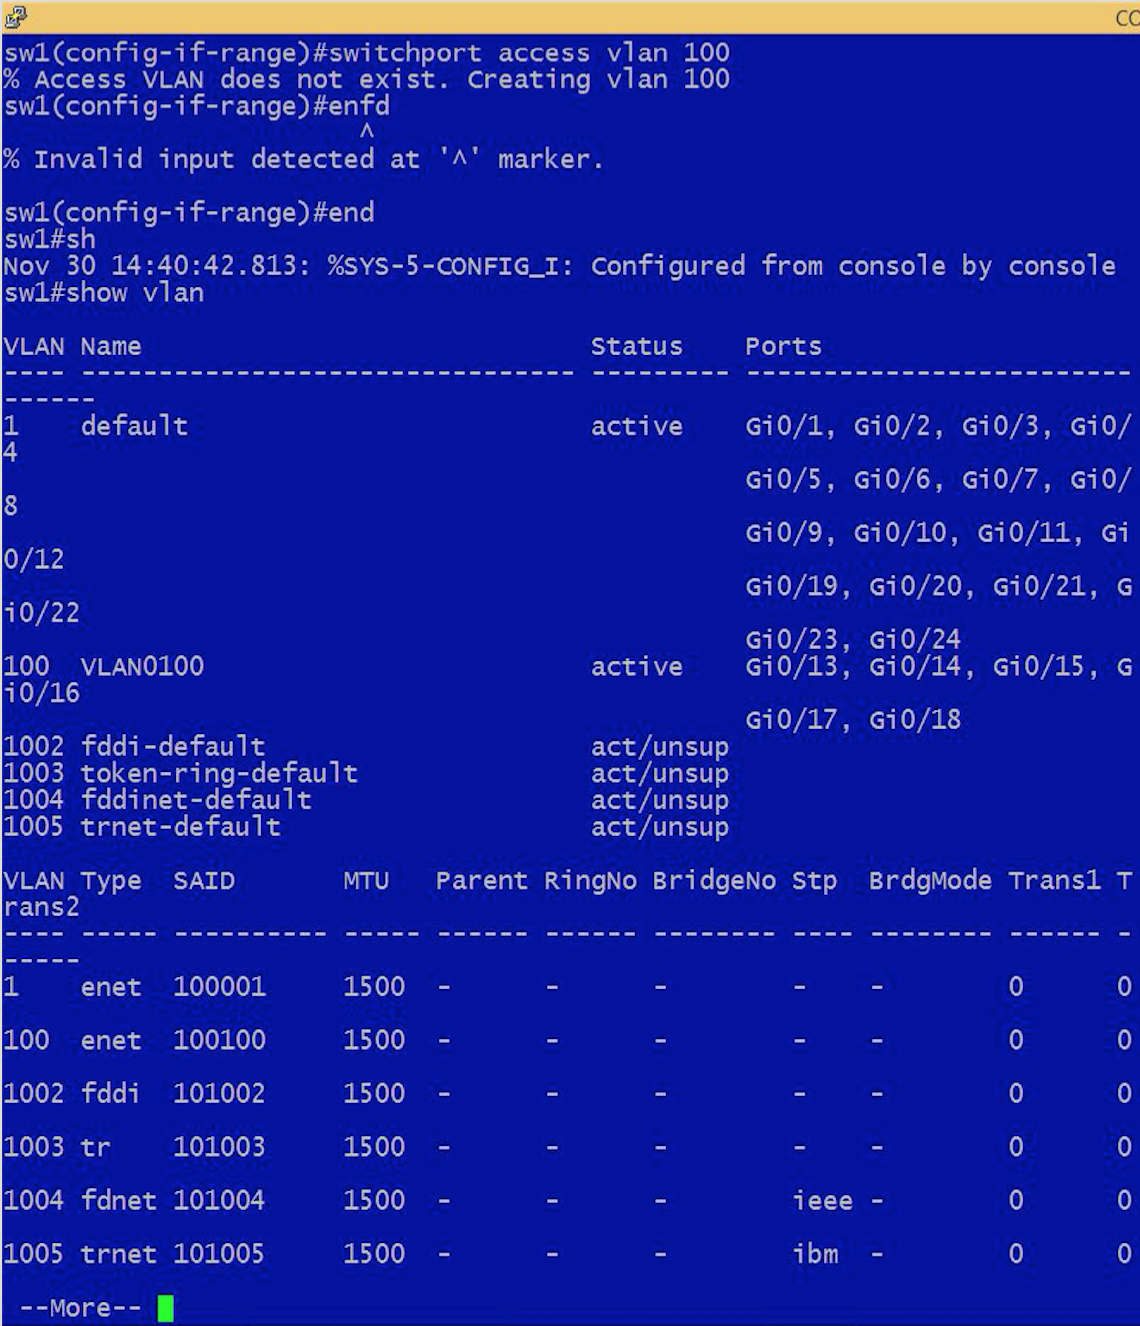
\includegraphics[width=15cm]{vlan}
    \label{fig:vlan}
    \end{figure}
    
    \item
    Die Kommunikaiton zwischen dem VLAN 100 und dem Default Bereich ist möglich, wenn die Kabelenden an den jeweiligen Bereichen eingesteckt sind.
    
    \item
    Es sind nun weitere Einträge in der Tabelle verzeichnet worden. Das VLAN und der Verbindungspunkt sind in der Tabelle eingetragen, außerdem wird angezeigt das dieser Switch die Root Bridge im VLAN 100 ist. Dieser VLAN hat nun seinen eigenen Spanning-Tree und die Ports von 13-18 sind nun für die anderen nicht mehr erreichbar.
    
    \item
    \textbf{KEINE NOTIZEN DAZU JEMAND ANDEREN FRAGEN ODER SVEN}
    
  \end{enumerate}
    
  \subsection[Aufgabe 8 VLAN-Trunk-Konfiguration]{VLAN-Trunk-Konfiguration}
    
  \renewcommand{\labelenumi}{\alph{enumi})}
  \begin{enumerate}
     \item
     Einstellungen vorgenommen.
     
     \begin{figure}
     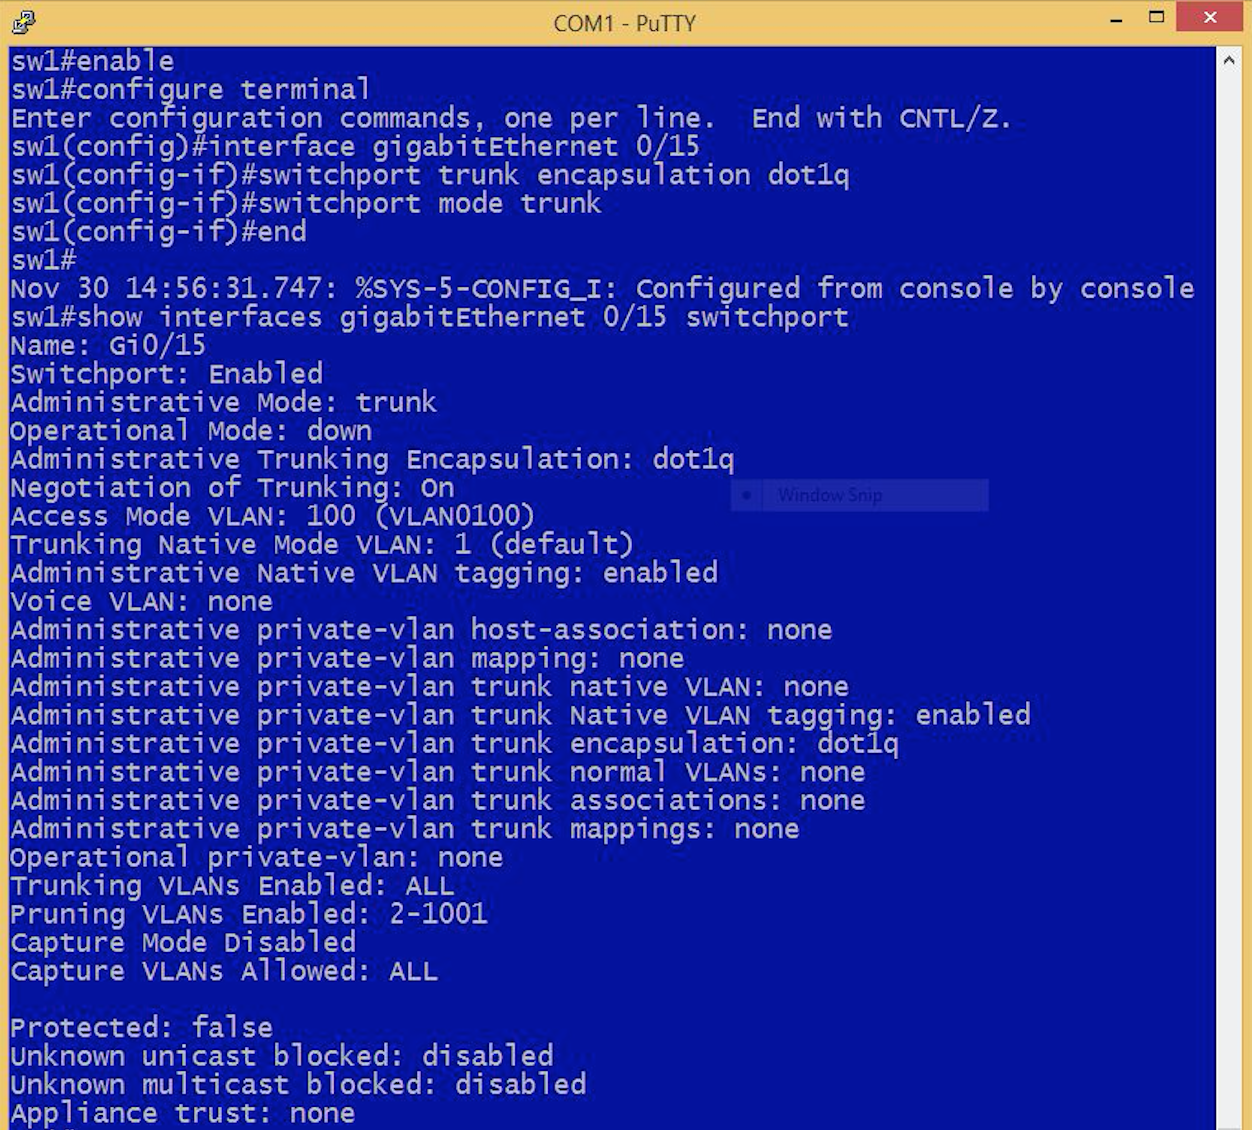
\includegraphics[width=10cm]{trunk}
     \label{fig:trunk}
     \end{figure}
     
     \item
     Das ''Trunking'' auf dem Interface \textit{gigabitEthernet 0/15} ist aktiviert und erlaubt.
     
     \item
     Die VLAN Tags die gefunden enthielten folgende Informationen:
     \begin{itemize}
     \item Priority
     \item CFI
     \item ID
     \item Ethernet Type/Length
     \end{itemize}
    
    \item
    Die Erreichbarkeit bleibt weiterhin behalten, jedoch haben sich die Portzustände bei einigen anderen Gruppen geändert.
    
    \item
    Um ein VLAN 200 zu konstruieren welches nur die LABPCs aller Teams vertritt, muss man nichts am ''Trunking'' verändern, weil diese automatisch generiert werden.
   \end{enumerate}
  
%----------------------------------------------------------------------------------------------------------------------------
  \newpage
\section[Versuch 5 Router]{Router}
  
  \subsection[Aufgabe 2 Traceroute (tracert)]{Traceroute (tracert)}
  \textbf{ANDERE FRAGEN WAS DIE HIERZU HABEN, ER HATTE UNS IN DER VORLESUNG JA I.WELCHE FRAGEN GESTELLT, DAS WÄRE GUT HIER}
  
  \subsection[Aufgabe 4 Erstellen der IP-Adressen für Interfaces und Netze]{Erstellen der IP-Adressen für Interfaces und Netze}
  
  \renewcommand{\labelenumi}{\alph{enumi})}
  \begin{enumerate}
  \item
  \textbf{wenn es bild dazu gibt hier einfügen, ansonsten blank}
  
  \item
  \textbf{dito a)}
  
  \item
  \textbf{dito a)}
  \end{enumerate}
  
  \subsection[Aufgabe 5 Konfiguration von DHCP zur dynamischen Adresszuweisung]{Konfiguration von DHCP zur dynamischen Adresszuweisung}
  
   \renewcommand{\labelenumi}{\alph{enumi})}
   \begin{enumerate}
   \item
   Die Subnetzmaske ist eine Bitmaske die zusammen mit der IP-Adresse, die Adresse einen Gerätes im Netz festlegt. Ein Subnetzmaske besteht aus 32-Bit und wir meisten in Kombination mit der IP-Adresse verwendet, deshalb ist sie auch genauso lang wie eine IP-Adresse. Die 32-Bit bestehen aus 24-Bit für das Netz und 8-Bit für den Host. Bei uns war diese \textit{255.255.0.0}.
   
   Der Standard-Gateway ist unser Router and den unsere Nachricht geschickt wird, falls die IP-Adresse an die wir senden wollen nicht im Subnetz befindet. Der Standard-Gateway überpüft dann ob die IP-Adresse in seinem Subnetz vorhanden ist, falls nicht wird das IP-Paket and die nächste Standard-Gateway geschickt. Dieser Vorgang wiederholt bis jemand das Netz der IP kennt und es dort hinschicken kann.

   \textbf{ÜBERPRÜF MAL OB MEINE ERKLÄRUNG SO PASST}   

   \item
   Einstellungen vorgenommen. \textbf{UNSERE BEFEHLE AUF DEM BILD HIGHLIGHTEN WENN SVEN SIE SCHICKT}
   
   \item
   \textbf{KEINE AHNUNG muss ich aus den Bildern entnehmen}
   
   \item
   \textbf{FALLS BILD VORHANDEN HIER EINFÜGEN}
   
   \item
   Um per DHCP eine bestimmte IP zuzuweisen, muss der Client vorher den Befehl \textit{''ipconfig/release''} ausführen. Dadurch wird die IP-Adresse für das angegebene Gerät oder das Gerät auf dem dieser Befehl ausgeführt wurde freigegeben. Mit dem Befehl \textit{''ipconfig/renew''} kann der Client nun erneut eine IP-Adresse anfordern.
   
   \item
   Es ist kein Router mit ping erreichbar und folgende Fehlermeldung wird zurückgegeben \textit{''host unreachable''}. Der Grund dafür ist das der Router ein eigenes Subnetz hat und die anderen Router in anderen Subnetzen sind. Somit kann unser Router die anderen Router nicht erreichen.
   
   Das ICMP-Protkoll dient zum Austausch von Informations- und Fehlermeldungen über das Internet Protokoll (IP). Dieses kann jedoch die Fehler nicht beheben, sondern nur eine Meldung an weitere Schichten geben. Eine mögliche Meldung könnte sein: \textit{''Echo Request''}.
   \end{enumerate}
   
   \subsection[Augabe 6 Konfiguration von OSPF als Routing-Protokoll]{Konfiguration von OSPF als Routing-Protokoll}
   
    \renewcommand{\labelenumi}{\alph{enumi})}
    \begin{enumerate}
    \item
    \textbf{MUSS ICH AUS DEM BILD ENTNEHMEN GEHT SCHNELL}
    
    \begin{table}
  \begin{tabular}{|l|l}
      \textbf{Protokollname} & \textbf{Vorlesung} \\ \hline
		 bla  & ja \\
		 bli  & nein \\
		 blub  & ja 
    \end{tabular}
     \caption{Prozesstabelle (BPDU-Pakete sind spezielle Pakete die Switches senden können)}
    \end{table}
    
    \item
    \textbf{HIER AUCH WENN BILD REIN DA SONST BLANK}
    
    \item
    Einstellungen vorgenommen.
    
    \item
    Durch das OSPF sind nun alle Router erreichbar und die Pingzeiten haben sich erheblich verbessert, alle sind unter einer Sekunde. 
    \textbf{AUS DEM BILD KANN ICH EVT MEHR ENTNNEHMEN}
    
    \item
    \textbf{AUS DEM BILD KANN ICH VLT WAS ENTNEHMEN}
    
    \item
    \textbf{AUS DEM BILD KANN ICH VLT WAS ENTNEHMEN, haben sich die Kosten verbessert?}
    
    \item
    \textbf{AUCH IM BILD NACHGUCKEN WELCHE BEFEHLE WIR BENUTZT HABEN}
    
    \item
    \textbf{MEHRERE SICHTWEISEN FRAGE ICH SVEN LIEBER NOCHMAL WAS ER DAZU DENKT }

    \end{enumerate}

  \subsection[Aufgabe 7 Auswirkungen IP-Paketlänge]{Auswirkungen IP-Paketlänge}
  
  \textbf{AUS DEM BILD ENTNEHMEN WENN ES EINS GIBT :D}
  
  \subsection{Untersuchungen zum Address Resolution Protocoll}
  
  \renewcommand{\labelenumi}{\alph{enumi})}
  \begin{enumerate}
  \item
  \textbf{WIEDER AUS DEM BILD ENTNEHMEN HAHA}
  
  \item
  \textbf{AUCH AUS DEM BILD ENTNEHMEN}
  
  \item
  \textbf{WAS SOLL ICH HIERZU DOKUMENTIEREN HANEMANN HAHAHA}
  \end{enumerate}    





%---------------------------------------------------------------------------------------------------------------------------- 
  \newpage
\section[Versuch 6 Transportschicht]{Transportschicht}
  
  
  
  
  
  
  
  
  
  
  
\end{document}